\documentclass{rapportENSIAS}
\usepackage{lipsum}
\usepackage{minted}
\definecolor{bg}{rgb}{0.95,0.95,0.95} % Couleur de fond des blocs de code

\usepackage{titlesec}  % Personnalisation des titres de chapitres / sections
\usepackage{tocloft}   % Personnalisation de la table des matières
\usepackage{hyperref}  % Liens hypertextes

% --- Packages additionnels utiles au rapport ---
\usepackage{booktabs}      % Tableaux de qualite (\toprule, \midrule, \bottomrule)
\usepackage{array}         % Colonnes de tableaux avancees
\usepackage{longtable}     % Tableaux sur plusieurs pages
\usepackage{multirow}      % Cellules fusionnees verticalement
\usepackage{xcolor}        % Couleurs
\usepackage{colortbl}      % Couleur de fond des cellules
\usepackage{graphicx}      % Images
\usepackage{float}         % Specificateur de position [H]
\usepackage{textcomp}      % Symboles additionnels (\textdegree)
\usepackage{tcolorbox}     % Boites colorees (info / succes / erreur)
\tcbuselibrary{skins,breakable}

% --- Palette de couleurs du rapport ---
\definecolor{qtblue}{HTML}{1F4E79}
\definecolor{qtcritique}{HTML}{C0392B}
\definecolor{qturgent}{HTML}{E67E22}
\definecolor{qtnonurgent}{HTML}{27AE60}
\definecolor{qtgray}{HTML}{ECECEC}

% --- Boites colorees reutilisables ---
\newtcolorbox{infobox}{colback=blue!5,colframe=qtblue,title=Information,fonttitle=\bfseries,breakable}
\newtcolorbox{successbox}{colback=green!5,colframe=qtnonurgent,title=Point cle,fonttitle=\bfseries,breakable}
\newtcolorbox{warningbox}{colback=red!5,colframe=qtcritique,title=Attention,fonttitle=\bfseries,breakable}

% --- Emplacement de figure (placeholder) lorsque l'image n'est pas encore disponible ---
\newcommand{\figplaceholder}[1]{%
  \begin{center}
  \setlength{\fboxsep}{10pt}%
  \fcolorbox{qtblue}{qtgray}{\parbox[c][4.2cm][c]{0.86\textwidth}{\centering\itshape #1}}%
  \end{center}%
}

\title{Rapport ENSIAS - QuickTriage}

\begin{document}

%----------- Informations du rapport ---------

\titre{QuickTriage : Système intelligent d'aide au triage des patients aux urgences par apprentissage automatique (KTAS)}
%\UE{UE PRO}
\sujet{Projet de Fin d'Année (PFA) -- Année universitaire 2025/2026}

\enseignant{Prénom \textsc{Nom} \textit{(encadrant·e à compléter)}}

\eleves{Ikram \textsc{Nom} \\
		Binôme \textsc{Nom} \textit{(éventuel)}}

\jury{ Prénom \textsc{Nom}\\
        Prénom \textsc{Nom}\\
    }

%----------- Initialisation -------------------

\fairemarges      % Afficher les marges
\fairepagedegarde % Creer la page de garde

%--------------les premieres pages--------------
\chapter*{Remerciements}
\addcontentsline{toc}{chapter}{Remerciements}

Au terme de ce projet de fin d'année, je tiens à exprimer ma profonde gratitude à
toutes les personnes qui ont contribué, de près ou de loin, à l'aboutissement de ce
travail.

Je remercie tout particulièrement mon encadrant·e, \textbf{Prénom \textsc{Nom}}, pour
la confiance accordée, la disponibilité, ainsi que pour les conseils avisés et les
orientations méthodologiques qui ont jalonné chacune des étapes de ce projet. Son
exigence bienveillante a constitué un moteur déterminant pour la qualité du résultat
final.

J'adresse également mes remerciements aux membres du jury, \textbf{Prénom \textsc{Nom}}
et \textbf{Prénom \textsc{Nom}}, qui m'ont fait l'honneur d'évaluer ce travail et dont
les remarques contribueront à l'enrichir.

Mes remerciements s'étendent au corps professoral et administratif de
\textbf{[établissement à compléter]} pour la qualité de la formation dispensée et pour
l'environnement propice à l'apprentissage et à l'innovation.

Enfin, je dédie une pensée reconnaissante à ma famille et à mes proches pour leur
soutien indéfectible tout au long de cette année universitaire.

\chapter*{Résumé}
\addcontentsline{toc}{chapter}{Résumé}

L'engorgement des services d'urgences hospitalières et la subjectivité inhérente au
triage manuel constituent des problématiques majeures de santé publique. Ce projet de
fin d'année présente \textbf{QuickTriage}, un système intelligent d'aide à la décision
destiné à soutenir le personnel soignant lors du triage des patients à leur arrivée.
À partir des paramètres vitaux mesurés (âge, état mental, douleur, pression artérielle,
fréquence cardiaque, fréquence respiratoire, température, saturation, etc.), le système
prédit automatiquement le niveau de priorité selon l'échelle \textbf{KTAS} (\textit{Korean
Triage and Acuity Scale}), regroupé en trois classes métier : \textsc{Critique},
\textsc{Urgent} et \textsc{Non urgent}.

La solution repose sur trois composantes complémentaires : (i) un pipeline
d'\textbf{apprentissage automatique} fondé sur un modèle \textbf{XGBoost} optimisé par
\textbf{Optuna}, entraîné sur un jeu de données réel augmenté de façon hybride
(SMOTE + génération calibrée) pour atteindre l'équilibre des classes ; (ii) un
\textbf{backend J2EE} (Jakarta EE / WildFly 10) exposant le modèle au format
\textbf{ONNX} via une API REST \textbf{JAX-RS} ; et (iii) un \textbf{frontend Flutter}
mobile pour la saisie des constantes et la lecture immédiate du niveau de priorité.

Une attention particulière a été portée à la détection et à la correction d'une fuite de
données (\textit{data leakage}), ainsi qu'à la calibration du seuil de décision en faveur
du rappel des cas graves. Le modèle final atteint une exactitude de \textbf{73,8~\%},
un \textbf{F1-score pondéré de 0,729} et un \textbf{rappel de 83,9~\%} sur la classe
\textsc{Critique}, garantissant une faible probabilité de sous-évaluer un patient en
danger vital.

\vspace{0.4cm}
\noindent\textbf{Mots-clés :} Triage médical, KTAS, aide à la décision clinique,
apprentissage automatique, XGBoost, ONNX, Jakarta EE, JAX-RS, Flutter, SMOTE, Optuna.

\chapter*{Abstract}
\addcontentsline{toc}{chapter}{Abstract}

Emergency department overcrowding and the subjectivity of manual triage are major public
health concerns. This end-of-year project introduces \textbf{QuickTriage}, an intelligent
decision-support system designed to assist healthcare staff during patient triage upon
arrival. Based on measured vital signs (age, mental status, pain, blood pressure, heart
rate, respiratory rate, body temperature, oxygen saturation, etc.), the system
automatically predicts the priority level according to the \textbf{KTAS} (Korean Triage
and Acuity Scale), grouped into three operational classes: \textsc{Critical},
\textsc{Urgent} and \textsc{Non-urgent}.

The solution relies on three complementary components: (i) a \textbf{machine learning}
pipeline based on an \textbf{XGBoost} model tuned with \textbf{Optuna}, trained on a real
dataset augmented through a hybrid strategy (SMOTE + calibrated synthetic generation) to
balance the classes; (ii) a \textbf{J2EE backend} (Jakarta EE / WildFly 10) exposing the
\textbf{ONNX} model through a \textbf{JAX-RS} REST API; and (iii) a mobile \textbf{Flutter}
frontend for entering vital signs and instantly reading the priority level.

Special care was given to detecting and correcting a \textit{data leakage} issue and to
calibrating the decision threshold in favour of recall for severe cases. The final model
reaches an accuracy of \textbf{73.8\%}, a \textbf{weighted F1-score of 0.729} and a
\textbf{recall of 83.9\%} on the \textsc{Critical} class, ensuring a low probability of
under-triaging life-threatening patients.

\vspace{0.4cm}
\noindent\textbf{Keywords:} Medical triage, KTAS, clinical decision support, machine
learning, XGBoost, ONNX, Jakarta EE, JAX-RS, Flutter, SMOTE, Optuna.

\chapter*{Liste des Abréviations}
\addcontentsline{toc}{chapter}{Liste des Abréviations}

\renewcommand{\arraystretch}{1.3}
\begin{longtable}{p{3.2cm} p{11cm}}
\toprule
\textbf{Abréviation} & \textbf{Signification} \\
\midrule
\endfirsthead
\toprule
\textbf{Abréviation} & \textbf{Signification} \\
\midrule
\endhead
KTAS      & \textit{Korean Triage and Acuity Scale} -- échelle coréenne de triage et d'acuité \\
CTAS      & \textit{Canadian Triage and Acuity Scale} \\
ESI       & \textit{Emergency Severity Index} \\
MTS       & \textit{Manchester Triage System} \\
ML        & \textit{Machine Learning} -- apprentissage automatique \\
IA        & Intelligence Artificielle \\
XGBoost   & \textit{eXtreme Gradient Boosting} \\
SMOTE     & \textit{Synthetic Minority Over-sampling Technique} \\
ONNX      & \textit{Open Neural Network Exchange} \\
API       & \textit{Application Programming Interface} \\
REST      & \textit{REpresentational State Transfer} \\
JAX-RS    & \textit{Jakarta API for RESTful Web Services} \\
EJB       & \textit{Enterprise JavaBeans} \\
J2EE      & \textit{Java 2 Platform, Enterprise Edition} / Jakarta EE \\
DTO       & \textit{Data Transfer Object} \\
JSON      & \textit{JavaScript Object Notation} \\
CSV       & \textit{Comma-Separated Values} \\
UML       & \textit{Unified Modeling Language} \\
UX/UI     & \textit{User eXperience / User Interface} \\
SBP       & \textit{Systolic Blood Pressure} -- pression artérielle systolique \\
DBP       & \textit{Diastolic Blood Pressure} -- pression artérielle diastolique \\
HR        & \textit{Heart Rate} -- fréquence cardiaque \\
RR        & \textit{Respiratory Rate} -- fréquence respiratoire \\
BT        & \textit{Body Temperature} -- température corporelle \\
NRS       & \textit{Numeric Rating Scale} -- échelle numérique d'évaluation de la douleur \\
SpO\textsubscript{2} & Saturation pulsée en oxygène \\
F1        & \textit{F1-score} (moyenne harmonique précision/rappel) \\
PFA       & Projet de Fin d'Année \\
\bottomrule
\end{longtable}

\newpage
\chapter*{Introduction générale}
\addcontentsline{toc}{chapter}{Introduction générale}

Les services d'urgences constituent la porte d'entrée principale du système hospitalier
et, à ce titre, sont soumis à une pression croissante. L'augmentation continue du nombre
de passages, conjuguée à la limitation des ressources humaines et matérielles, engendre
un phénomène d'engorgement aux conséquences directes sur la qualité des soins et sur la
sécurité des patients. Dans ce contexte, le \textit{triage} -- c'est-à-dire la
hiérarchisation des patients selon la gravité de leur état -- joue un rôle déterminant :
il s'agit d'orienter, dans un temps très court, les patients les plus critiques vers une
prise en charge immédiate tout en organisant l'attente des cas moins urgents.

Or, le triage demeure dans de nombreux établissements une opération manuelle, dépendante
de l'expérience et de la disponibilité du personnel soignant. Cette subjectivité expose
à deux types d'erreurs : la \textit{sur-évaluation} (mobiliser inutilement des ressources)
et surtout la \textit{sous-évaluation} (sous-estimer un patient réellement en danger), cette
dernière étant la plus lourde de conséquences. L'apport des méthodes d'apprentissage
automatique, capables d'objectiver et d'accélérer cette décision à partir des paramètres
vitaux, apparaît dès lors comme une piste prometteuse.

C'est précisément l'ambition du projet \textbf{QuickTriage} : concevoir un outil d'aide
à la décision qui prédit automatiquement le niveau de priorité KTAS d'un patient à partir
de ses constantes, sans jamais se substituer au jugement clinique du soignant, qui
conserve toujours la décision finale. Ce rapport décrit la démarche complète, depuis
l'analyse du besoin jusqu'à l'implémentation, en passant par la conception logicielle et
la modélisation du système.

Le présent document est organisé en six chapitres. Le \textbf{chapitre~1} pose le contexte
général, la problématique et les objectifs. Le \textbf{chapitre~2} dresse un état de l'art
des systèmes de triage et positionne QuickTriage. Le \textbf{chapitre~3} formalise
l'analyse et la spécification des besoins. Le \textbf{chapitre~4} présente la conception et
l'architecture du système. Le \textbf{chapitre~5} détaille la modélisation UML. Enfin, le
\textbf{chapitre~6} expose l'implémentation et la démonstration de la solution, avant la
conclusion générale et les perspectives.

%------------
\newpage
\tabledematieres % Creer la table des matieres

\newpage
\listoffigures

\newpage
\listoftables

%------------ Corps du rapport ----------------
\chapter{Contexte Général du Projet}

\section*{Introduction du chapitre}
Ce premier chapitre a pour vocation de planter le décor du projet \textbf{QuickTriage}.
Il s'agit de comprendre l'environnement dans lequel s'inscrit la solution, à savoir le
fonctionnement des services d'urgences hospitalières et les difficultés structurelles
auxquelles ils font face. Après avoir exposé le contexte et la problématique, nous
présenterons la motivation qui a guidé ce travail, puis nous formaliserons les objectifs,
principal et spécifiques. Le chapitre se clôt par la mise en évidence des contributions et
des innovations apportées par QuickTriage.

\section{Contexte et Problématique}

\subsection{Le triage aux urgences : une fonction critique}
Le service des urgences est, par définition, un environnement où l'incertitude et le
caractère vital des décisions cohabitent en permanence. À leur arrivée, les patients
présentent des tableaux cliniques extrêmement hétérogènes, allant du motif bénin à
l'urgence vitale. Le \textit{triage} consiste à évaluer rapidement la gravité de chaque
patient afin de déterminer l'ordre et le délai de prise en charge. Cette étape, réalisée
généralement par un infirmier organisateur de l'accueil (IOA), conditionne l'ensemble du
parcours de soins : un triage juste sauve des vies, un triage erroné peut être fatal.

\subsection{L'engorgement des urgences}
Partout dans le monde, les services d'urgences connaissent une croissance soutenue du
nombre de passages, sans augmentation proportionnelle des moyens. Cet
\textit{engorgement} se traduit par des temps d'attente allongés, une saturation des box
de soins et une charge mentale accrue pour le personnel. Dans un tel contexte, la pression
temporelle pesant sur la décision de triage augmente, et avec elle le risque d'erreur.
La rapidité et la fiabilité de l'évaluation initiale deviennent des enjeux de premier plan.

\subsection{Les limites du triage manuel}
Le triage manuel, bien qu'encadré par des échelles standardisées, demeure tributaire de
plusieurs facteurs de variabilité :
\begin{itemize}
  \item \textbf{La subjectivité de l'évaluateur} : deux soignants peuvent attribuer des
  niveaux différents à un même patient, en fonction de leur expérience et de leur état de
  fatigue.
  \item \textbf{La pression temporelle} : la nécessité de décider vite favorise les biais
  cognitifs et les raccourcis de raisonnement.
  \item \textbf{La charge cognitive} : l'intégration mentale simultanée de nombreux
  paramètres vitaux est difficile, surtout en période d'affluence.
  \item \textbf{Le risque de sous-triage} : sous-estimer la gravité d'un patient constitue
  l'erreur la plus dangereuse, car elle retarde une prise en charge potentiellement vitale.
\end{itemize}

\begin{warningbox}
Le \textit{sous-triage} (classer un patient grave comme non urgent) est l'erreur la plus
redoutée en médecine d'urgence. La conception de QuickTriage place donc la maximisation du
\textbf{rappel sur la classe \textsc{Critique}} au cœur de ses priorités, quitte à tolérer
quelques sur-triages.
\end{warningbox}

\subsection{Énoncé de la problématique}
La problématique centrale de ce projet peut être formulée ainsi : \textit{Comment concevoir
un outil numérique fiable, rapide et accessible, capable d'assister le personnel soignant
dans la décision de triage en objectivant l'évaluation de la priorité d'un patient à partir
de ses paramètres vitaux, tout en garantissant que la décision clinique finale demeure de la
responsabilité du soignant~?}

\section{Motivation du Projet}
La motivation du projet QuickTriage procède d'un triple constat. D'abord, un
\textbf{constat clinique} : les erreurs de triage, et singulièrement le sous-triage,
demeurent une cause évitable de morbidité. Ensuite, un \textbf{constat technologique} :
les progrès récents de l'apprentissage automatique, conjugués à des formats d'échange de
modèles interopérables comme ONNX et à des frameworks mobiles modernes comme Flutter,
rendent désormais réaliste le déploiement d'un outil d'aide à la décision léger et
embarquable. Enfin, un \textbf{constat d'opportunité} : il existe des jeux de données
publics de triage (notamment basés sur l'échelle KTAS) permettant d'entraîner et de valider
de tels modèles.

L'ambition n'est pas de remplacer le soignant, mais de lui offrir un \textbf{second avis
objectif et instantané}, agissant comme un filet de sécurité contre les erreurs
d'inattention et comme un accélérateur de la décision en période de forte affluence.

\section{Objectifs}

\subsection{Objectif principal}
L'objectif principal est de \textbf{concevoir et réaliser un système complet d'aide au
triage} qui prédit automatiquement le niveau de priorité KTAS d'un patient à partir de ses
constantes vitales, et le restitue de manière claire et immédiate au personnel soignant via
une application mobile.

\subsection{Objectifs spécifiques}
\begin{enumerate}
  \item \textbf{Construire un modèle d'apprentissage automatique} robuste de classification
  du niveau KTAS, en traitant explicitement les difficultés de qualité des données (fuite de
  données, déséquilibre des classes).
  \item \textbf{Maximiser le rappel de la classe \textsc{Critique}} afin de minimiser le
  sous-triage, par une calibration adaptée du seuil de décision.
  \item \textbf{Exposer le modèle via une API REST} performante et interopérable, en
  s'appuyant sur le format ONNX et une architecture J2EE (Jakarta EE / WildFly).
  \item \textbf{Développer une application mobile Flutter} ergonomique, optimisée pour une
  saisie rapide et une lecture immédiate du résultat (code couleur de priorité).
  \item \textbf{Garantir la primauté du jugement clinique}, le système se positionnant
  strictement comme une aide à la décision et non comme un décideur autonome.
\end{enumerate}

\section{Contributions et Innovations}
Au-delà de l'assemblage de briques technologiques, le projet QuickTriage se distingue par
plusieurs contributions :
\begin{itemize}
  \item \textbf{Diagnostic et correction d'une fuite de données.} Une première version du
  modèle s'appuyait sur un jeu de données contenant une variable (\texttt{plasma\_glucose})
  introduisant une fuite de données (\textit{data leakage}). Sa détection a conduit à un
  changement de jeu de données vers \textit{KTAS Emergency Triage}, gage de résultats
  honnêtes et généralisables.
  \item \textbf{Stratégie d'augmentation hybride des données.} Pour pallier le déséquilibre
  des classes, une approche combinant la génération de patients synthétiques calibrés sur la
  distribution réelle et l'algorithme SMOTE (avec \texttt{k\_neighbors} adaptatif) a été mise
  en œuvre, aboutissant à un jeu équilibré de 3~000 patients (600 par classe).
  \item \textbf{Calibration orientée sécurité patient.} Le seuil de décision de la classe
  \textsc{Critique} a été abaissé à 0,30 afin de privilégier le rappel des cas graves, en
  cohérence avec l'impératif clinique de limiter le sous-triage.
  \item \textbf{Chaîne d'intégration interopérable.} L'export du modèle au format ONNX et son
  chargement unique au démarrage du serveur J2EE assurent des inférences rapides et
  reproductibles, indépendamment du langage d'entraînement.
\end{itemize}

\begin{successbox}
QuickTriage n'est pas un simple prototype de modèle~: c'est une \textbf{chaîne complète et
cohérente}, de la donnée brute jusqu'à l'application mobile, dont chaque maillon a été
pensé pour la fiabilité et la sécurité du patient.
\end{successbox}

\section*{Conclusion du chapitre}
Ce chapitre a permis de cerner le contexte du triage aux urgences, d'en exposer les limites
actuelles et de formuler la problématique à laquelle QuickTriage entend répondre. Nous avons
également défini les objectifs du projet et mis en lumière ses principales contributions.
Pour situer notre solution par rapport à l'existant et en justifier les choix, le chapitre
suivant propose un état de l'art des systèmes de triage et un positionnement comparatif de
QuickTriage.

\chapter{État de l'Art et Positionnement}

\section*{Introduction du chapitre}
Avant de concevoir une nouvelle solution, il est indispensable d'examiner les approches
existantes afin d'en comprendre les forces, les limites et les zones d'innovation possibles.
Ce chapitre dresse d'abord un panorama des principales échelles de triage normalisées
(CTAS, ESI, MTS, KTAS), puis des outils logiciels et des travaux de recherche mobilisant
l'apprentissage automatique pour le triage. Il se conclut par une analyse comparative
positionnant QuickTriage au regard de ces solutions.

\section{Analyse des solutions existantes}

\subsection{Les échelles de triage normalisées}
Afin de réduire la variabilité du triage, plusieurs échelles standardisées à cinq niveaux
ont été développées et largement adoptées à l'échelle internationale.

\begin{itemize}
  \item \textbf{CTAS} (\textit{Canadian Triage and Acuity Scale}) : échelle canadienne à
  cinq niveaux, associant à chaque niveau un délai cible de prise en charge ; elle s'appuie
  sur des plaintes types et des modificateurs (paramètres vitaux, douleur).
  \item \textbf{ESI} (\textit{Emergency Severity Index}) : échelle nord-américaine à cinq
  niveaux fondée sur un algorithme décisionnel qui combine la gravité immédiate et la
  consommation prévisible de ressources.
  \item \textbf{MTS} (\textit{Manchester Triage System}) : système britannique reposant sur
  des organigrammes (\textit{flowcharts}) par motif de consultation, aboutissant à un code
  couleur de priorité.
  \item \textbf{KTAS} (\textit{Korean Triage and Acuity Scale}) : adaptation coréenne de la
  CTAS, également à cinq niveaux, qui sert de référence à ce projet. Le niveau~1 correspond à
  une urgence vitale immédiate et le niveau~5 à un cas non urgent.
\end{itemize}

Le tableau~\ref{tab:echelles} synthétise les caractéristiques de ces échelles.

\begin{table}[h]
\centering
\renewcommand{\arraystretch}{1.3}
\begin{tabular}{p{2.2cm} p{2.2cm} p{2cm} p{6.5cm}}
\toprule
\textbf{Échelle} & \textbf{Origine} & \textbf{Niveaux} & \textbf{Principe de fonctionnement} \\
\midrule
CTAS & Canada & 5 & Plaintes types + modificateurs (constantes, douleur) \\
ESI  & États-Unis & 5 & Algorithme gravité + ressources prévisibles \\
MTS  & Royaume-Uni & 5 & Organigrammes par motif, code couleur \\
KTAS & Corée du Sud & 5 & Adaptation de la CTAS, niveau 1 = urgence vitale \\
\bottomrule
\end{tabular}
\caption{Comparaison des principales échelles de triage normalisées.}
\label{tab:echelles}
\end{table}

\subsection{Le regroupement métier adopté par QuickTriage}
Si l'échelle KTAS comporte cinq niveaux, l'usage opérationnel de triage privilégie souvent
un regroupement plus lisible. QuickTriage adopte un regroupement en \textbf{trois classes
métier}, présenté au tableau~\ref{tab:classes}, qui simplifie la lecture tout en préservant
l'essentiel de l'information clinique : la distinction entre l'urgence vitale, l'urgence
relative et le non-urgent.

\begin{table}[h]
\centering
\renewcommand{\arraystretch}{1.4}
\begin{tabular}{p{3.2cm} p{2.5cm} p{6.5cm}}
\toprule
\textbf{Classe métier} & \textbf{Niveaux KTAS} & \textbf{Délai de prise en charge} \\
\midrule
\textcolor{qtcritique}{\textbf{CRITIQUE}}     & KTAS 1--2 & Prise en charge immédiate ($<$ 15 min) \\
\textcolor{qturgent}{\textbf{URGENT}}         & KTAS 3    & Prise en charge rapide \\
\textcolor{qtnonurgent}{\textbf{NON\_URGENT}} & KTAS 4--5 & Prise en charge différée \\
\bottomrule
\end{tabular}
\caption{Regroupement des niveaux KTAS en trois classes métier dans QuickTriage.}
\label{tab:classes}
\end{table}

\subsection{Outils logiciels existants}
Sur le plan logiciel, l'informatisation du triage prend aujourd'hui plusieurs formes :
\begin{itemize}
  \item \textbf{Modules de triage intégrés aux DPI} (dossiers patients informatisés) : ils
  guident la saisie selon une échelle (souvent ESI ou MTS) mais reposent essentiellement sur
  des règles fixes et l'appréciation humaine, sans réelle prédiction statistique.
  \item \textbf{Calculateurs et applications de scores} : applications mobiles reproduisant
  les organigrammes d'une échelle donnée ; elles guident le soignant mais n'apprennent pas
  des données.
  \item \textbf{Solutions de recherche fondées sur l'IA} : prototypes académiques explorant
  des modèles prédictifs, rarement intégrés dans une chaîne applicative complète et
  déployable.
\end{itemize}

\subsection{Approches d'apprentissage automatique dans la littérature}
La littérature scientifique sur le triage assisté par apprentissage automatique a connu un
essor notable. Les travaux mobilisent typiquement des modèles tels que la régression
logistique, les forêts aléatoires, les machines à gradient boosté (dont XGBoost) ou encore
les réseaux de neurones, à partir des paramètres vitaux et de variables administratives. Les
principaux enseignements de ces travaux, qui ont guidé nos choix, sont les suivants :
\begin{itemize}
  \item Les méthodes d'\textbf{ensemble par boosting} (XGBoost et apparentés) offrent un
  excellent compromis entre performance et robustesse sur des données tabulaires
  hétérogènes.
  \item Le \textbf{déséquilibre des classes} (les cas critiques étant rares) constitue un
  obstacle majeur, justifiant des techniques de rééquilibrage telles que SMOTE.
  \item L'\textbf{évaluation} ne doit pas se limiter à l'exactitude globale ; le rappel sur
  les classes graves est l'indicateur de sécurité déterminant.
  \item La \textbf{fuite de données} est un piège fréquent qui conduit à surestimer
  artificiellement les performances ; sa détection est cruciale.
\end{itemize}

\section{Analyse comparative et positionnement de QuickTriage}

\subsection{Critères de comparaison}
Pour positionner QuickTriage, nous retenons les critères suivants : l'échelle de triage
utilisée, le degré d'automatisation, le recours effectif à l'apprentissage automatique,
l'intégration dans une application mobile, la prise en compte de la sécurité patient
(orientation vers le rappel des cas graves), et la complétude de la chaîne applicative
(de la donnée jusqu'au déploiement).

\subsection{Tableau comparatif}
Le tableau~\ref{tab:positionnement} confronte QuickTriage aux grandes familles de solutions
identifiées.

\begin{table}[h]
\centering
\renewcommand{\arraystretch}{1.4}
\small
\begin{tabular}{p{3.2cm} p{2.3cm} p{2.3cm} p{2.3cm} p{3.2cm}}
\toprule
\textbf{Critère} & \textbf{Échelles manuelles} & \textbf{Modules DPI} & \textbf{Protos IA (recherche)} & \textbf{QuickTriage} \\
\midrule
Échelle utilisée        & Variable & ESI/MTS & Variable & KTAS (3 classes) \\
Automatisation          & Aucune & Partielle (règles) & Modèle seul & De bout en bout \\
Apprentissage auto.     & Non & Non & Oui & Oui (XGBoost+Optuna) \\
Intégration mobile      & Non & Rare & Rare & Oui (Flutter) \\
Orientation sécurité    & Dépend de l'humain & Règles fixes & Variable & Rappel CRITIQUE optimisé \\
Chaîne complète         & --- & Partielle & Non & ML + J2EE + Mobile \\
\bottomrule
\end{tabular}
\caption{Positionnement comparatif de QuickTriage.}
\label{tab:positionnement}
\end{table}

\subsection{Synthèse du positionnement}
Il ressort de cette analyse que QuickTriage se distingue moins par l'emploi isolé d'une
technique que par la \textbf{cohérence et la complétude de sa chaîne}. Là où les outils
existants se cantonnent souvent à une seule dimension -- guidage par règles, ou modèle
prédictif sans intégration -- QuickTriage articule un pipeline d'apprentissage rigoureux
(détection de fuite, rééquilibrage, optimisation, calibration), une exposition
interopérable via ONNX et une API REST J2EE, ainsi qu'une application mobile pensée pour le
terrain. Surtout, le projet assume un parti pris clair de \textbf{sécurité patient} en
optimisant le rappel des cas critiques, ce qui le différencie des approches purement
orientées exactitude globale.

\section*{Conclusion du chapitre}
Cet état de l'art a permis de situer les échelles de triage de référence, de recenser les
outils existants et de dégager les enseignements de la littérature sur l'apprentissage
automatique appliqué au triage. Le positionnement comparatif a mis en évidence la valeur
ajoutée de QuickTriage : une solution intégrée, interopérable et orientée sécurité patient.
Forts de ce cadrage, nous pouvons désormais formaliser précisément les besoins du système,
objet du chapitre suivant.

\chapter{Analyse et Spécification des Besoins}

\section*{Introduction du chapitre}
La réussite d'un projet logiciel repose sur une compréhension fine et formalisée des
besoins. Ce chapitre présente la démarche d'analyse adoptée, identifie les acteurs du
système et leurs rôles, puis détaille les besoins fonctionnels et non-fonctionnels de
QuickTriage. Il se conclut par la présentation de la méthodologie de gestion de projet
retenue, accompagnée de sa planification.

\section{Étude des besoins}

\subsection{Méthodologie d'analyse}
L'analyse des besoins a été conduite selon une démarche itérative et centrée utilisateur.
Elle s'est appuyée sur trois leviers : (i) l'étude du domaine métier (fonctionnement du
triage, échelle KTAS, contraintes des urgences) ; (ii) l'analyse des données disponibles
afin de vérifier la faisabilité de la prédiction ; et (iii) la projection des scénarios
d'usage sur le terrain, pour garantir l'adéquation de l'outil aux contraintes réelles du
soignant (rapidité, lisibilité, fiabilité). Les besoins ainsi recueillis ont été classés en
besoins fonctionnels (ce que le système doit faire) et non-fonctionnels (les qualités
attendues).

\subsection{Acteurs du système}
Trois acteurs principaux interagissent avec QuickTriage. Le tableau~\ref{tab:acteurs} en
précise les rôles.

\begin{table}[h]
\centering
\renewcommand{\arraystretch}{1.4}
\begin{tabular}{p{4cm} p{10cm}}
\toprule
\textbf{Acteur} & \textbf{Rôle et responsabilités} \\
\midrule
\textbf{Personnel soignant / Infirmier de tri} & Acteur principal. Saisit les constantes
vitales du patient, déclenche la prédiction, consulte le niveau de priorité proposé et la
confiance associée. Reste le décideur final du triage. \\
\textbf{Médecin} & Valide ou corrige la proposition du système, supervise les cas critiques
et exploite l'information de priorité pour organiser la prise en charge. \\
\textbf{Administrateur} & Gère la configuration technique (déploiement du modèle, version,
paramètres), assure la maintenance et le suivi du bon fonctionnement du système. \\
\bottomrule
\end{tabular}
\caption{Acteurs du système QuickTriage et leurs rôles.}
\label{tab:acteurs}
\end{table}

\begin{infobox}
QuickTriage est explicitement un \textbf{outil d'aide à la décision}. Le niveau KTAS proposé
est une recommandation ; la responsabilité du triage demeure celle du personnel soignant et
du médecin.
\end{infobox}

\section{Besoins fonctionnels}
Les besoins fonctionnels décrivent les services que le système doit rendre. Ils sont
synthétisés dans le tableau~\ref{tab:bf}.

\begin{table}[h]
\centering
\renewcommand{\arraystretch}{1.3}
\begin{tabular}{p{1.6cm} p{4.2cm} p{8cm}}
\toprule
\textbf{Réf.} & \textbf{Besoin} & \textbf{Description} \\
\midrule
BF1 & Saisie des constantes & Permettre la saisie rapide des paramètres vitaux du patient
(âge, état mental, douleur/NRS, SBP, DBP, HR, RR, BT, saturation, mode d'arrivée, etc.). \\
BF2 & Prédiction du niveau KTAS & Calculer automatiquement la classe de priorité
(CRITIQUE / URGENT / NON\_URGENT) à partir des constantes saisies. \\
BF3 & Affichage du résultat & Restituer la classe prédite, le délai maximal associé et le
niveau de confiance, avec un code couleur de priorité. \\
BF4 & Indicateur de criticité & Signaler explicitement les cas critiques
(\texttt{isCritical}) pour attirer l'attention du soignant. \\
BF5 & Détail des probabilités & Afficher la répartition des probabilités entre les trois
classes pour une lecture nuancée. \\
BF6 & Validation clinique & Permettre au soignant/médecin de valider ou corriger la
proposition. \\
BF7 & Historique des triages & Conserver une trace des évaluations réalisées (consultation
ultérieure). \\
BF8 & Gestion de version du modèle & Exposer la version du modèle utilisé
(\texttt{modelVersion}) pour la traçabilité. \\
\bottomrule
\end{tabular}
\caption{Besoins fonctionnels de QuickTriage.}
\label{tab:bf}
\end{table}

\section{Besoins non-fonctionnels}
Les besoins non-fonctionnels expriment les qualités attendues du système. Compte tenu du
domaine médical, ils revêtent une importance particulière.

\begin{table}[h]
\centering
\renewcommand{\arraystretch}{1.3}
\begin{tabular}{p{3.2cm} p{10.6cm}}
\toprule
\textbf{Catégorie} & \textbf{Exigence} \\
\midrule
\textbf{Performance / Latence} & L'inférence doit être quasi instantanée (chargement unique
du modèle ONNX au démarrage, réponse de l'API en deçà de quelques centaines de
millisecondes). \\
\textbf{Fiabilité} & Le système doit fournir des prédictions stables et reproductibles ;
priorité au rappel des cas CRITIQUES pour limiter le sous-triage. \\
\textbf{Sécurité des données} & Les données de santé étant sensibles, l'accès à l'API doit
être protégé, les échanges sécurisés (HTTPS) et la collecte minimisée. \\
\textbf{Utilisabilité} & Interface mobile claire, saisie rapide, lecture immédiate du
résultat grâce au code couleur, adaptée à un usage sous pression. \\
\textbf{Scalabilité} & Architecture capable d'absorber des montées en charge (statelessness
des services EJB, modèle chargé en singleton). \\
\textbf{Maintenabilité} & Code modulaire, séparation nette des couches (ML, backend,
frontend), métadonnées de prétraitement externalisées pour faciliter les mises à jour du
modèle. \\
\textbf{Interopérabilité} & Recours au format ONNX et à une API REST standard pour
découpler l'entraînement du déploiement. \\
\bottomrule
\end{tabular}
\caption{Besoins non-fonctionnels de QuickTriage.}
\label{tab:bnf}
\end{table}

\section{Méthodologie de gestion de projet}

\subsection{Choix et justification}
Compte tenu de la nature exploratoire du volet \textit{data science} (où les résultats
d'une étape conditionnent les choix de la suivante) et du besoin d'itérations fréquentes,
une démarche \textbf{agile et incrémentale} a été retenue. Le projet a été découpé en
incréments livrables, chacun apportant une valeur vérifiable : préparation des données,
modèle de référence, optimisation, intégration backend, application mobile. Cette approche a
notamment permis de réagir rapidement à la découverte de la fuite de données, en
réorientant le projet vers un nouveau jeu de données sans remettre en cause l'ensemble de la
planification.

\subsection{Planification}
La figure~\ref{fig:gantt} présente le diagramme de Gantt synthétisant le déroulement du
projet sur la période considérée. Les grandes phases s'enchaînent tout en autorisant des
recouvrements (par exemple, le début de l'intégration backend pendant l'affinage du
modèle).

\begin{figure}[h]
\centering
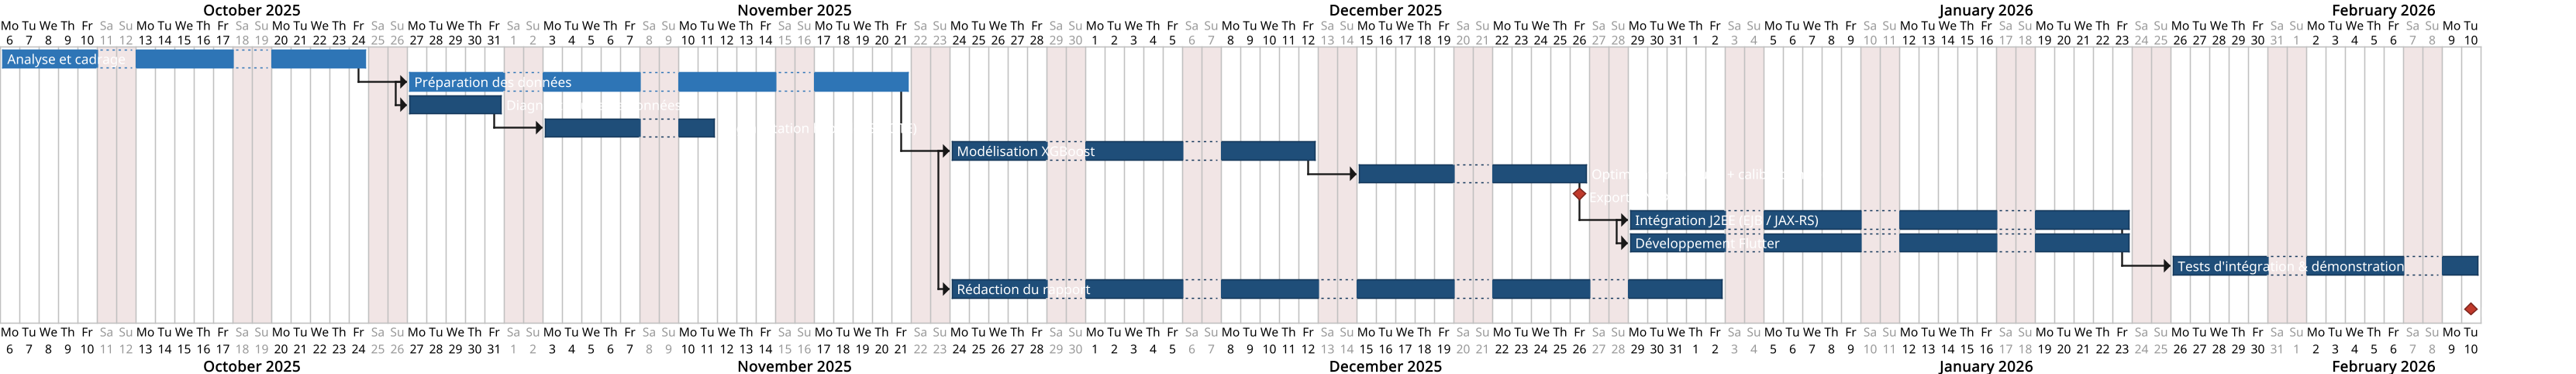
\includegraphics[width=\textwidth]{images/gantt.png}
\caption{Diagramme de Gantt du projet QuickTriage.}
\label{fig:gantt}
\end{figure}

\noindent Les principales phases sont les suivantes :
\begin{enumerate}
  \item \textbf{Analyse et cadrage} : étude du domaine, des échelles de triage et des
  besoins.
  \item \textbf{Préparation des données} : exploration, diagnostic de la fuite de données,
  changement de jeu de données, nettoyage, augmentation hybride.
  \item \textbf{Modélisation} : entraînement du modèle de référence puis du modèle XGBoost.
  \item \textbf{Optimisation et calibration} : recherche d'hyperparamètres avec Optuna,
  calibration du seuil de la classe CRITIQUE.
  \item \textbf{Intégration backend} : export ONNX, chargement du modèle, services EJB, API
  REST JAX-RS.
  \item \textbf{Développement frontend} : application mobile Flutter et consommation de
  l'API.
  \item \textbf{Tests, démonstration et rédaction} : validation de bout en bout et
  documentation.
\end{enumerate}

\section*{Conclusion du chapitre}
Ce chapitre a formalisé les besoins de QuickTriage : identification des acteurs, besoins
fonctionnels et non-fonctionnels, puis méthodologie de gestion de projet et planification.
Ces spécifications constituent le socle sur lequel reposera la conception. Le chapitre
suivant traduit ces besoins en une architecture système cohérente, articulant les couches
machine learning, backend et frontend.

\chapter{Conception et Architecture Système}

\section*{Introduction du chapitre}
Après avoir formalisé les besoins, ce chapitre traduit les exigences de QuickTriage en une
architecture logicielle cohérente. Nous présentons d'abord l'architecture générale en
couches, puis nous détaillons chacune des composantes : le pipeline de données et
d'apprentissage, le backend J2EE exposant le modèle, et le frontend mobile Flutter. Une
section est consacrée à la sécurité des données de santé, particulièrement sensible dans le
domaine médical. Le chapitre se conclut par les choix d'expérience et d'interface
utilisateur (UX/UI).

\section{Architecture générale du système}

\subsection{Vue d'ensemble en trois couches}
QuickTriage adopte une architecture en trois couches faiblement couplées, organisée autour
d'un principe directeur : \textbf{découpler l'entraînement du modèle de son déploiement}.
Cette séparation permet de faire évoluer indépendamment le modèle d'apprentissage, la logique
applicative et l'interface utilisateur. Les trois couches sont les suivantes :

\begin{enumerate}
  \item \textbf{La couche d'apprentissage automatique (\textit{offline}).} Réalisée en
  Python, elle prend en charge la préparation des données, l'entraînement, l'optimisation et
  la calibration du modèle. Son livrable est un artefact interopérable au format \textbf{ONNX}
  accompagné de ses métadonnées de prétraitement.
  \item \textbf{La couche backend (\textit{serveur d'application}).} Réalisée en Jakarta EE et
  déployée sur \textbf{WildFly~10}, elle charge le modèle ONNX, applique le même prétraitement
  qu'à l'entraînement, exécute l'inférence et expose le service via une API REST
  \textbf{JAX-RS}.
  \item \textbf{La couche frontend (\textit{client mobile}).} Réalisée en \textbf{Flutter},
  elle assure la saisie des constantes vitales, l'appel à l'API et la restitution visuelle du
  résultat au personnel soignant.
\end{enumerate}

\begin{infobox}
La frontière nette entre la phase \textit{offline} (entraînement Python) et la phase
\textit{online} (inférence Java) est rendue possible par le format ONNX, qui sérialise le
modèle de façon indépendante du langage. Le serveur Java n'a ainsi aucune dépendance vis-à-vis
de Python à l'exécution.
\end{infobox}

\subsection{Flux global de l'information}
Le cheminement d'une requête de triage illustre l'articulation des couches : le soignant
saisit les constantes dans l'application Flutter ; celles-ci sont sérialisées en JSON et
transmises par requête HTTP \texttt{POST} à l'API REST ; le backend désérialise la requête,
reconstruit le vecteur de caractéristiques, applique l'imputation et la standardisation, puis
exécute l'inférence ONNX ; le résultat (classe, confiance, probabilités, indicateur de
criticité) est renvoyé en JSON et affiché à l'écran avec un code couleur de priorité. Le
tableau~\ref{tab:couches} synthétise les responsabilités et technologies de chaque couche.

\begin{table}[h]
\centering
\renewcommand{\arraystretch}{1.4}
\begin{tabular}{p{3cm} p{5.5cm} p{5cm}}
\toprule
\textbf{Couche} & \textbf{Responsabilités} & \textbf{Technologies} \\
\midrule
Apprentissage (offline) & Préparation, entraînement, optimisation, calibration, export &
Python, pandas, scikit-learn, XGBoost, Optuna, SMOTE, ONNX \\
Backend (serveur) & Chargement du modèle, prétraitement, inférence, exposition REST &
Jakarta EE, WildFly 10, JAX-RS, EJB, ONNX Runtime \\
Frontend (mobile) & Saisie, validation, appel API, restitution visuelle &
Flutter, Dart, HTTP \\
\bottomrule
\end{tabular}
\caption{Responsabilités et technologies des trois couches de QuickTriage.}
\label{tab:couches}
\end{table}

\section{Architecture de données et pipeline d'apprentissage}

\subsection{Du jeu de données brut au modèle déployable}
La couche d'apprentissage suit un pipeline séquentiel dont chaque étape produit un artefact
exploitable par la suivante. Ce pipeline, conçu pour être reproductible, comprend :

\begin{enumerate}
  \item \textbf{Acquisition et diagnostic.} Chargement du jeu de données \textit{KTAS
  Emergency Triage} (1~267 patients réels) et contrôle de qualité, incluant la détection de
  toute variable susceptible d'introduire une fuite de données.
  \item \textbf{Nettoyage et prétraitement.} Traitement des valeurs manquantes par imputation
  (médianes), encodage des variables catégorielles et construction du vecteur de
  caractéristiques (23 \textit{features}).
  \item \textbf{Augmentation hybride.} Rééquilibrage des classes par combinaison de génération
  synthétique calibrée et de l'algorithme SMOTE, aboutissant à un jeu équilibré de 3~000
  patients (600 par classe).
  \item \textbf{Standardisation.} Normalisation des variables par \textit{StandardScaler}
  (centrage-réduction), dont les paramètres (moyennes, écarts-types) sont sauvegardés.
  \item \textbf{Entraînement et optimisation.} Apprentissage d'un modèle XGBoost dont les
  hyperparamètres sont optimisés par Optuna.
  \item \textbf{Calibration et évaluation.} Réglage du seuil de décision de la classe
  \textsc{Critique} et évaluation orientée sécurité patient (rappel des cas graves).
  \item \textbf{Export.} Sérialisation du modèle au format ONNX et externalisation des
  métadonnées de prétraitement dans un fichier JSON.
\end{enumerate}

\subsection{Externalisation des métadonnées de prétraitement}
Un choix de conception déterminant consiste à \textbf{externaliser les paramètres de
prétraitement} dans un fichier \texttt{metadata\_v3.json} plutôt que de les coder en dur. Ce
fichier contient les moyennes et écarts-types du \textit{StandardScaler}, les médianes de
l'imputeur, le seuil de la classe \textsc{Critique} (0,30) et la version du modèle. Le backend
le charge au démarrage, garantissant ainsi que \textbf{le prétraitement appliqué à l'inférence
est rigoureusement identique à celui de l'entraînement}. Cette cohérence est essentielle :
toute divergence de normalisation entre l'entraînement et l'inférence dégraderait silencieusement
les performances.

\begin{successbox}
L'externalisation des métadonnées dans \texttt{metadata\_v3.json} permet de mettre à jour le
modèle (nouvel ONNX + nouvelles métadonnées) \textbf{sans recompiler le backend}, améliorant
nettement la maintenabilité de la chaîne.
\end{successbox}

\section{Architecture du backend J2EE}

\subsection{Organisation en composants}
Le backend repose sur trois composants Jakarta EE aux responsabilités clairement séparées,
selon une logique de couches (présentation REST, logique métier, accès au modèle) :

\begin{itemize}
  \item \texttt{OnnxModelLoader} -- un bean \textbf{\texttt{@Singleton @Startup}} chargé une
  seule fois à l'amorçage du serveur. Il instancie l'environnement et la session ONNX Runtime
  et les maintient en mémoire pendant toute la durée de vie de l'application.
  \item \texttt{TriagePredictionService} -- un EJB \textbf{\texttt{@Stateless}} qui porte la
  logique métier : construction du vecteur de caractéristiques, imputation, standardisation,
  appel à la session ONNX et application du seuil de criticité.
  \item \texttt{TriageResource} -- une ressource \textbf{JAX-RS} (\texttt{@Path
  "/api/triage"}) qui expose le point d'entrée REST \texttt{POST /predict}, désérialise la
  requête JSON et sérialise la réponse.
\end{itemize}

\subsection{Justification des choix d'architecture}
Le recours au patron \textbf{Singleton} pour le chargement du modèle répond à une exigence de
performance : le chargement d'un modèle ONNX et l'initialisation du \textit{runtime} sont des
opérations coûteuses qu'il serait inacceptable de répéter à chaque requête. En les réalisant
une seule fois au démarrage, on garantit une inférence quasi instantanée par la suite. Le
caractère \textbf{\texttt{@Stateless}} du service métier favorise la scalabilité : le conteneur
peut instancier autant de beans que nécessaire pour traiter les requêtes concurrentes, sans
état partagé à synchroniser. Enfin, l'exposition via \textbf{JAX-RS} assure l'interopérabilité
et le découplage vis-à-vis du client mobile, conformément aux besoins non-fonctionnels.

\subsection{Contrat d'interface REST}
L'API expose un point d'entrée principal, décrit au tableau~\ref{tab:rest}. L'échange repose
sur le format JSON, standard et léger, adapté à une consommation mobile.

\begin{table}[h]
\centering
\renewcommand{\arraystretch}{1.4}
\begin{tabular}{p{2cm} p{4cm} p{7.5cm}}
\toprule
\textbf{Méthode} & \textbf{Chemin} & \textbf{Description} \\
\midrule
\texttt{POST} & \texttt{/api/triage/predict} & Reçoit les constantes vitales
(\texttt{TriageRequest}) et retourne la classe KTAS prédite, la confiance, les probabilités
par classe et l'indicateur de criticité (\texttt{TriageResponse}). \\
\bottomrule
\end{tabular}
\caption{Point d'entrée principal de l'API REST de QuickTriage.}
\label{tab:rest}
\end{table}

\section{Sécurité des données de santé}
Les données manipulées par QuickTriage relèvent de la catégorie des \textbf{données de santé},
particulièrement sensibles et soumises à des exigences réglementaires strictes (par exemple le
RGPD en Europe). La conception intègre donc plusieurs principes de protection, en cohérence avec
les recommandations \textbf{OWASP} :

\begin{itemize}
  \item \textbf{Minimisation des données.} Seules les constantes strictement nécessaires à la
  prédiction sont collectées ; aucune donnée d'identification directe du patient n'est requise
  pour l'inférence.
  \item \textbf{Chiffrement des échanges.} Les communications entre l'application mobile et le
  backend doivent emprunter le protocole \textbf{HTTPS}, afin de protéger les données en transit.
  \item \textbf{Contrôle d'accès.} L'accès à l'API doit être restreint au personnel autorisé,
  via un mécanisme d'authentification (jetons), conformément au principe du moindre privilège.
  \item \textbf{Validation des entrées.} Les données reçues sont systématiquement validées
  (bornes physiologiques, types) afin de prévenir les injections et les requêtes malformées.
  \item \textbf{Traçabilité.} L'historisation des décisions de triage (horodatage, version du
  modèle, décision finale) assure l'auditabilité du système.
\end{itemize}

\begin{warningbox}
La sécurité n'est pas une option dans un système médical. La protection des données en transit
(HTTPS), le contrôle d'accès et la validation des entrées constituent le socle minimal de toute
mise en production de QuickTriage.
\end{warningbox}

\section{Conception de l'expérience et de l'interface utilisateur}

\subsection{Principes directeurs}
L'interface de QuickTriage est conçue pour un usage \textbf{sous pression}, dans un
environnement où chaque seconde compte. Trois principes guident sa conception :
\begin{itemize}
  \item \textbf{Rapidité de saisie} : des champs ordonnés selon le flux naturel de recueil des
  constantes, des claviers numériques adaptés et des valeurs par défaut raisonnables.
  \item \textbf{Lisibilité immédiate du résultat} : un \textbf{code couleur de priorité}
  (rouge pour \textsc{Critique}, orange pour \textsc{Urgent}, vert pour \textsc{Non urgent})
  permettant une lecture instantanée, complété par le délai maximal et le niveau de confiance.
  \item \textbf{Confiance et transparence} : l'affichage des probabilités par classe et de la
  version du modèle donne au soignant les éléments pour exercer son jugement critique sur la
  proposition.
\end{itemize}

\subsection{Code couleur et hiérarchie visuelle}
Le code couleur reprend les conventions du triage hospitalier afin de ne pas dérouter le
personnel. La hiérarchie visuelle met en avant l'information la plus critique (la classe et,
le cas échéant, l'alerte de criticité), reléguant les détails (probabilités, métadonnées) à un
second plan consultable à la demande. Ce parti pris réduit la charge cognitive et accélère la
décision.

\section*{Conclusion du chapitre}
Ce chapitre a présenté l'architecture en trois couches de QuickTriage et justifié ses choix
structurants : découplage entraînement/déploiement via ONNX, externalisation des métadonnées
de prétraitement, composants J2EE aux responsabilités séparées, sécurisation des données de
santé et interface orientée terrain. Cette architecture constitue le squelette de la solution.
Le chapitre suivant en propose une vue formelle au travers de la modélisation UML : cas
d'utilisation, diagramme de classes et scénarios de séquence.

\chapter{Modélisation UML et Conception Détaillée}

\section*{Introduction du chapitre}
La modélisation UML (\textit{Unified Modeling Language}) offre une représentation formelle et
normalisée de la structure et du comportement du système. Ce chapitre détaille la conception de
QuickTriage à travers trois familles de diagrammes complémentaires : le diagramme de cas
d'utilisation, qui décrit les interactions des acteurs avec le système ; le diagramme de
classes, qui en présente la structure statique ; et trois diagrammes de séquence, qui en
illustrent le comportement dynamique sur des scénarios représentatifs.

\section{Diagramme de cas d'utilisation}

\subsection{Présentation}
Le diagramme de cas d'utilisation (figure~\ref{fig:usecase}) recense les fonctionnalités
offertes par QuickTriage et les associe aux trois acteurs identifiés au chapitre~3 :
l'infirmier de tri, le médecin et l'administrateur.

\begin{figure}[h]
\centering
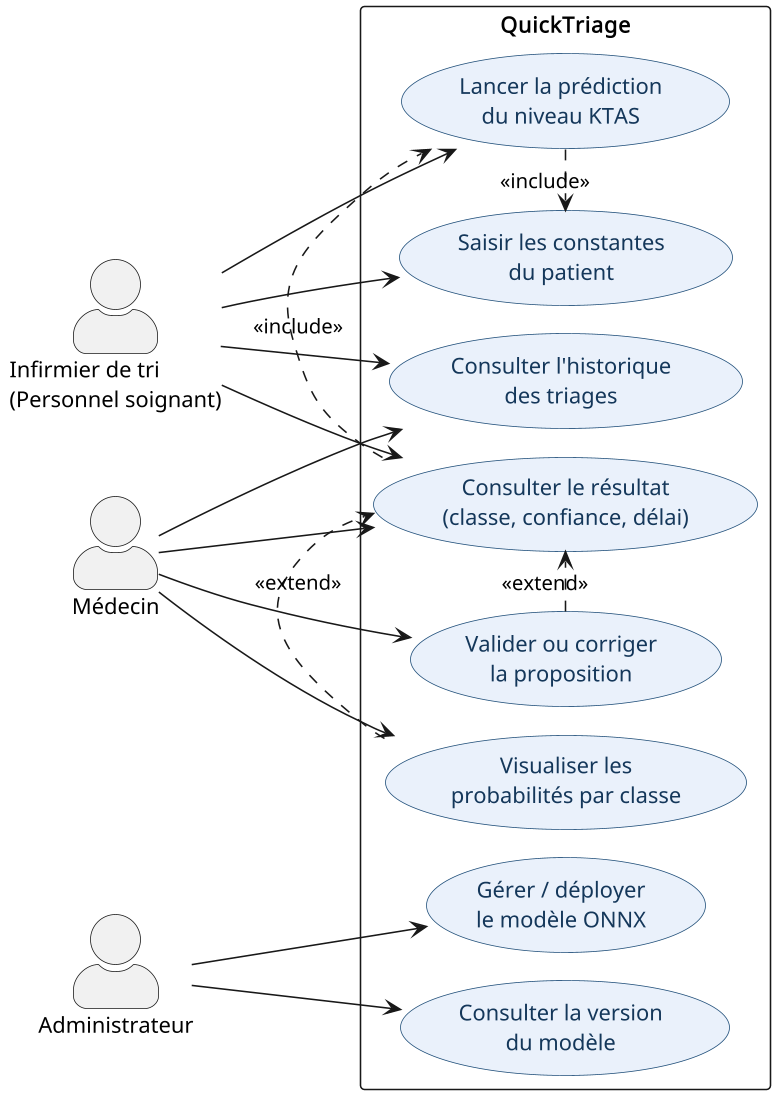
\includegraphics[width=0.95\textwidth]{images/usecase.png}
\caption{Diagramme de cas d'utilisation global de QuickTriage.}
\label{fig:usecase}
\end{figure}

\subsection{Analyse}
L'\textbf{infirmier de tri}, acteur principal, concentre le cœur du parcours opérationnel :
saisir les constantes, lancer la prédiction, consulter le résultat et accéder à l'historique.
Le \textbf{médecin} intervient en supervision : il consulte le résultat, visualise le détail
des probabilités et valide ou corrige la proposition du système. L'\textbf{administrateur}
prend en charge les tâches techniques : déploiement du modèle ONNX et consultation de sa
version.

Les relations entre cas d'utilisation précisent la logique fonctionnelle. La relation
\texttt{<<include>>} entre « Lancer la prédiction » et « Saisir les constantes » traduit le
fait que la prédiction présuppose nécessairement une saisie préalable ; de même, « Consulter le
résultat » inclut la prédiction. Les relations \texttt{<<extend>>} reliant « Visualiser les
probabilités » et « Valider ou corriger » à « Consulter le résultat » expriment des
comportements optionnels, déclenchés à la discrétion de l'utilisateur. Cette structuration
garantit que l'acte de triage reste rapide par défaut, tout en autorisant un approfondissement
sur demande.

\section{Diagramme de classes}

\subsection{Présentation}
Le diagramme de classes (figure~\ref{fig:classes}) décrit la structure statique de la solution,
en distinguant les composants du backend J2EE et les modèles du frontend Flutter.

\begin{figure}[h]
\centering
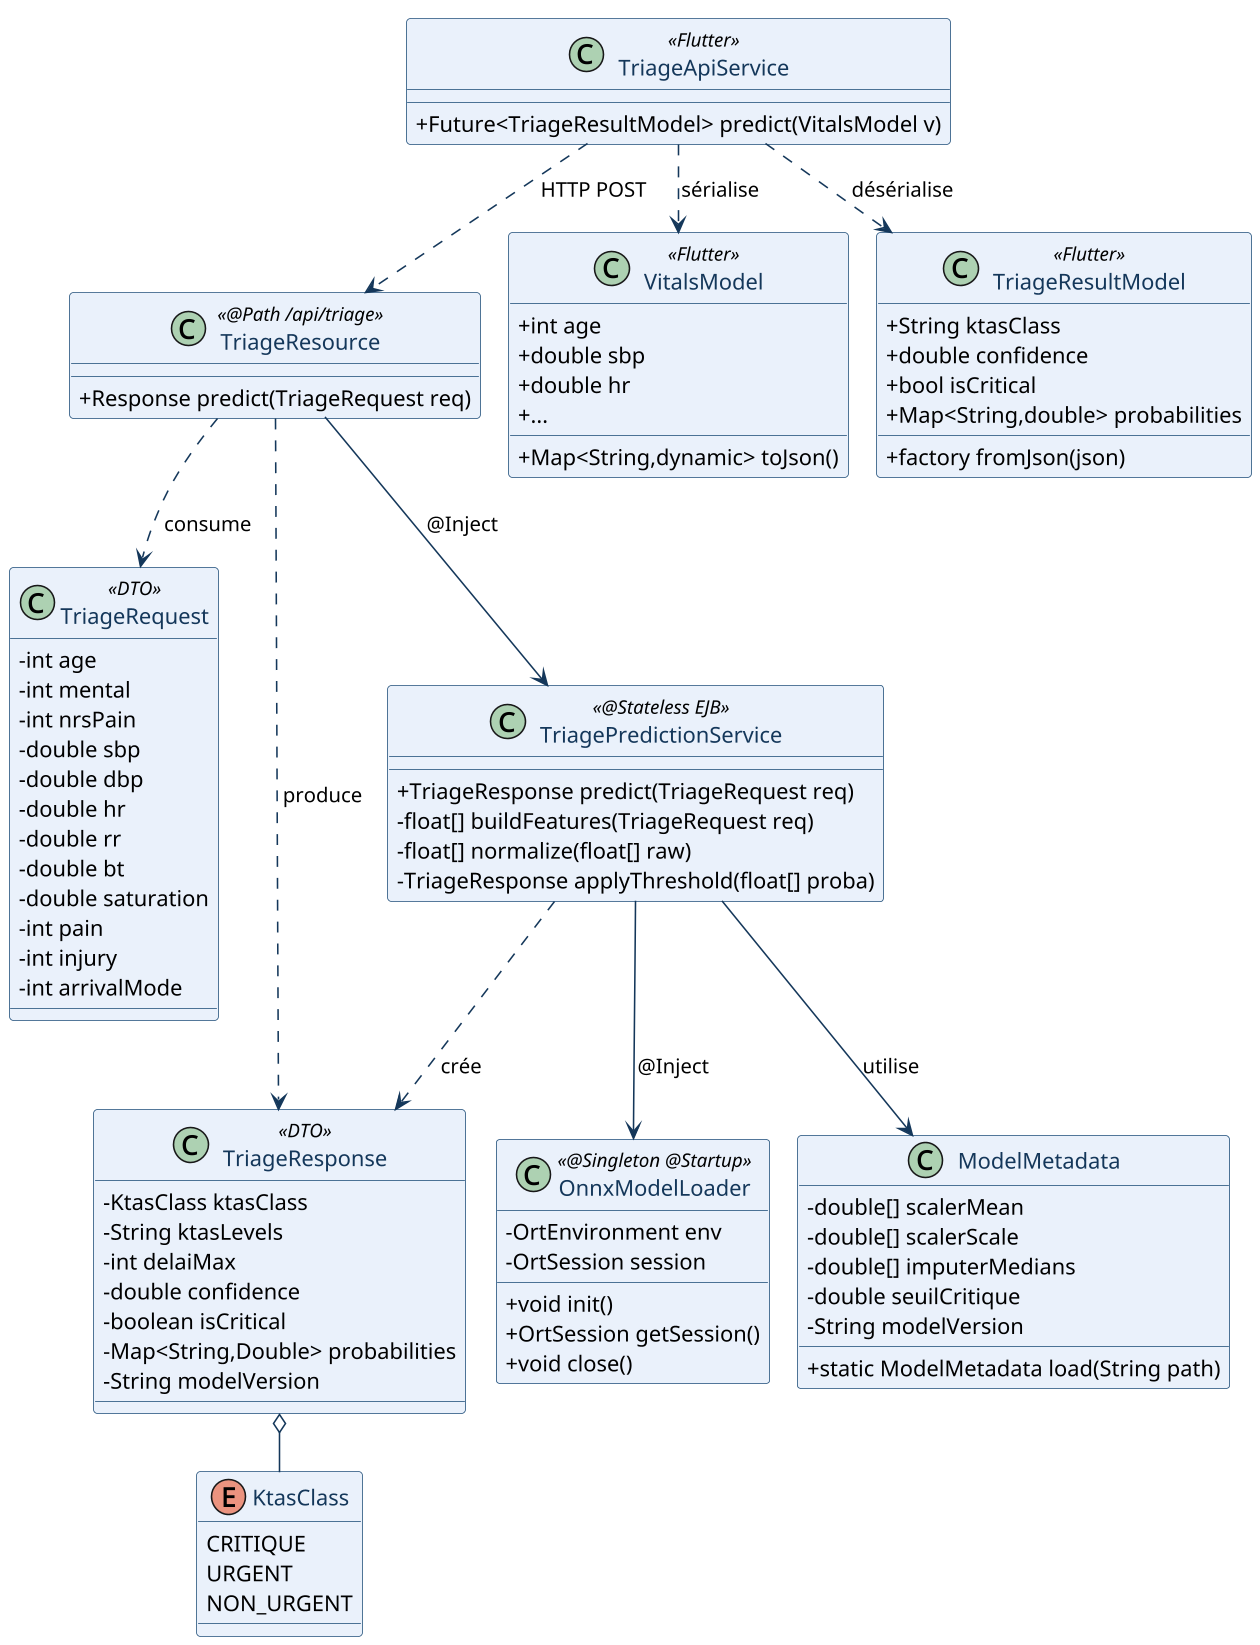
\includegraphics[width=\textwidth]{images/class.png}
\caption{Diagramme de classes de QuickTriage (backend J2EE et modèles frontend).}
\label{fig:classes}
\end{figure}

\subsection{Analyse des classes du backend}
Le backend s'organise autour de cinq classes et d'une énumération :
\begin{itemize}
  \item \texttt{TriageRequest} et \texttt{TriageResponse} sont des \textbf{DTO}
  (\textit{Data Transfer Objects}). Le premier transporte les constantes vitales saisies
  (âge, état mental, douleur, SBP, DBP, HR, RR, BT, saturation, etc.) ; le second véhicule le
  résultat (classe KTAS, délai maximal, confiance, indicateur \texttt{isCritical}, probabilités
  par classe et version du modèle).
  \item \texttt{TriageResource} est la ressource \textbf{JAX-RS} (\texttt{@Path /api/triage})
  qui consomme un \texttt{TriageRequest} et produit un \texttt{TriageResponse}. Elle délègue le
  traitement au service métier.
  \item \texttt{TriagePredictionService} est l'\textbf{EJB \texttt{@Stateless}} qui orchestre
  la prédiction : \texttt{buildFeatures()} construit le vecteur, \texttt{normalize()} applique
  la standardisation et \texttt{applyThreshold()} décide de la classe selon le seuil de
  criticité.
  \item \texttt{OnnxModelLoader} est le bean \textbf{\texttt{@Singleton @Startup}} qui détient
  l'\texttt{OrtEnvironment} et l'\texttt{OrtSession}, initialisés une fois au démarrage et
  exposés via \texttt{getSession()}.
  \item \texttt{ModelMetadata} encapsule les paramètres de prétraitement chargés depuis
  \texttt{metadata\_v3.json} (moyennes et écarts-types du scaler, médianes de l'imputeur, seuil
  de la classe \textsc{Critique}, version du modèle).
  \item L'énumération \texttt{KtasClass} matérialise les trois classes métier : \texttt{CRITIQUE},
  \texttt{URGENT} et \texttt{NON\_URGENT}.
\end{itemize}

Les associations traduisent les dépendances d'injection (\texttt{@Inject}) : la ressource
dépend du service, qui dépend lui-même du chargeur de modèle et exploite les métadonnées. Ce
graphe de dépendances reflète fidèlement la séparation des responsabilités décrite au
chapitre~4.

\subsection{Analyse des modèles du frontend}
Côté Flutter, trois classes assurent le miroir client : \texttt{VitalsModel} représente les
constantes saisies et fournit une méthode \texttt{toJson()} de sérialisation ;
\texttt{TriageResultModel} représente le résultat et propose une fabrique \texttt{fromJson()}
de désérialisation ; \texttt{TriageApiService} encapsule l'appel HTTP \texttt{POST} vers la
ressource REST, sérialisant la requête et désérialisant la réponse. Cette symétrie entre les
DTO du backend et les modèles du frontend garantit un contrat d'échange clair et maintenable.

\section{Diagrammes de séquence}
Les diagrammes de séquence décrivent les interactions temporelles entre les objets pour trois
scénarios représentatifs : le cycle complet d'une demande de triage, le détail de l'appel REST
et de l'inférence, et la validation clinique avec historisation.

\subsection{Scénario 1 : cycle complet d'une demande de triage}
Le premier scénario (figure~\ref{fig:seqtriage}) retrace le parcours nominal de bout en bout,
depuis la saisie des constantes par l'infirmier jusqu'à l'affichage du résultat coloré.

\begin{figure}[h]
\centering
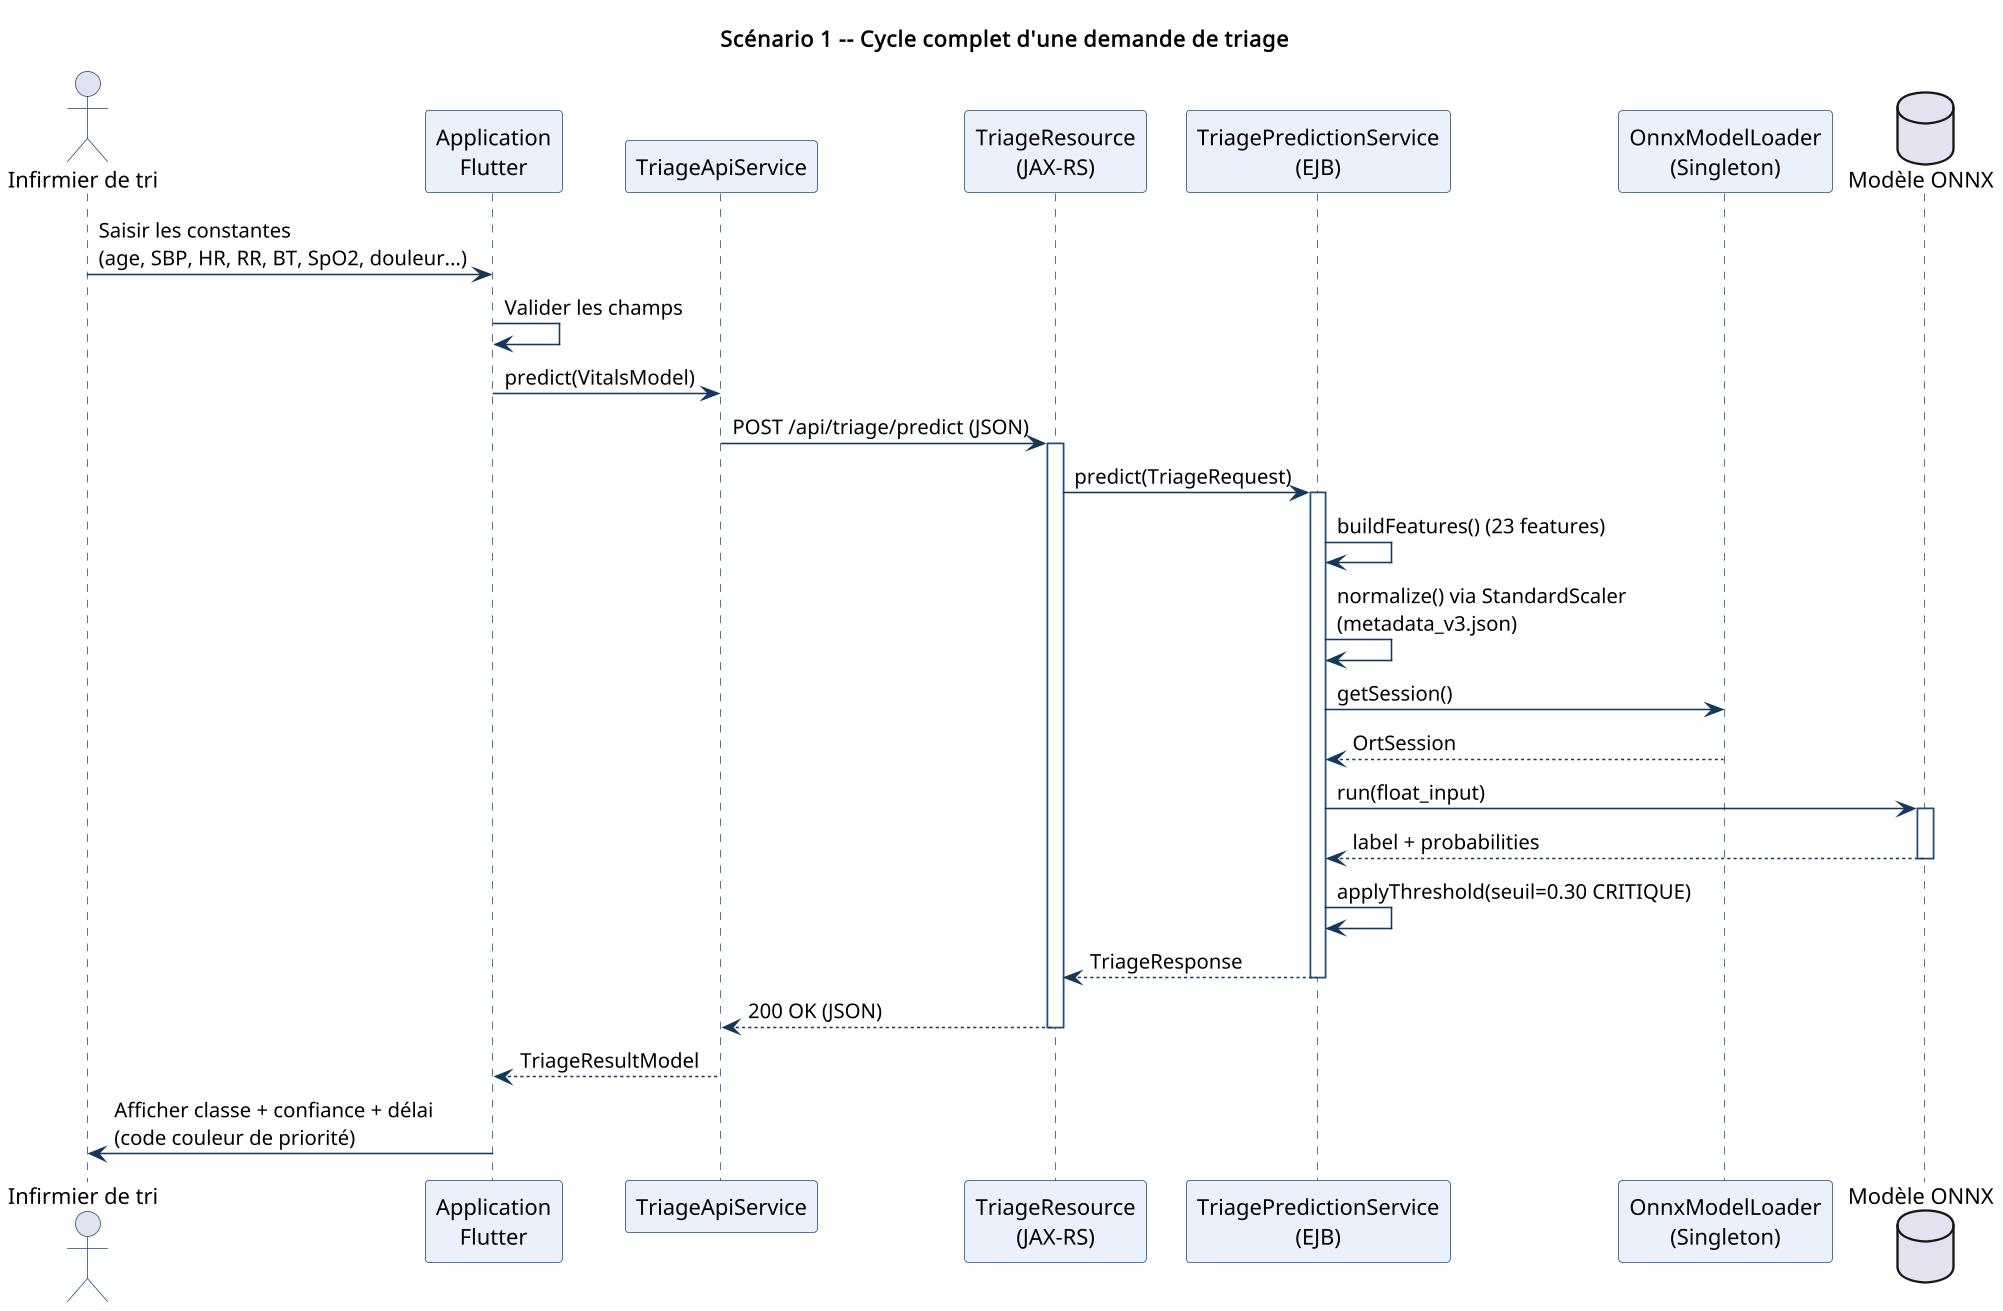
\includegraphics[width=\textwidth]{images/seq_triage.png}
\caption{Scénario 1 -- Cycle complet d'une demande de triage.}
\label{fig:seqtriage}
\end{figure}

\noindent Ce diagramme met en évidence la chaîne d'appels : l'application Flutter valide les
champs puis invoque \texttt{TriageApiService}, qui émet une requête \texttt{POST} vers
\texttt{TriageResource}. Le service métier construit et normalise les caractéristiques, sollicite
la session ONNX maintenue par \texttt{OnnxModelLoader}, applique le seuil de criticité (0,30 pour
la classe \textsc{Critique}) et retourne la réponse. Le résultat remonte jusqu'à l'interface, où
il est affiché avec le code couleur de priorité. On observe que le chargement du modèle n'apparaît
pas dans ce flux : il a eu lieu une fois pour toutes au démarrage du serveur.

\subsection{Scénario 2 : traitement de la requête REST et inférence ONNX}
Le deuxième scénario (figure~\ref{fig:seqrest}) zoome sur le traitement côté backend, en
détaillant les étapes de prétraitement et la logique de décision.

\begin{figure}[h]
\centering
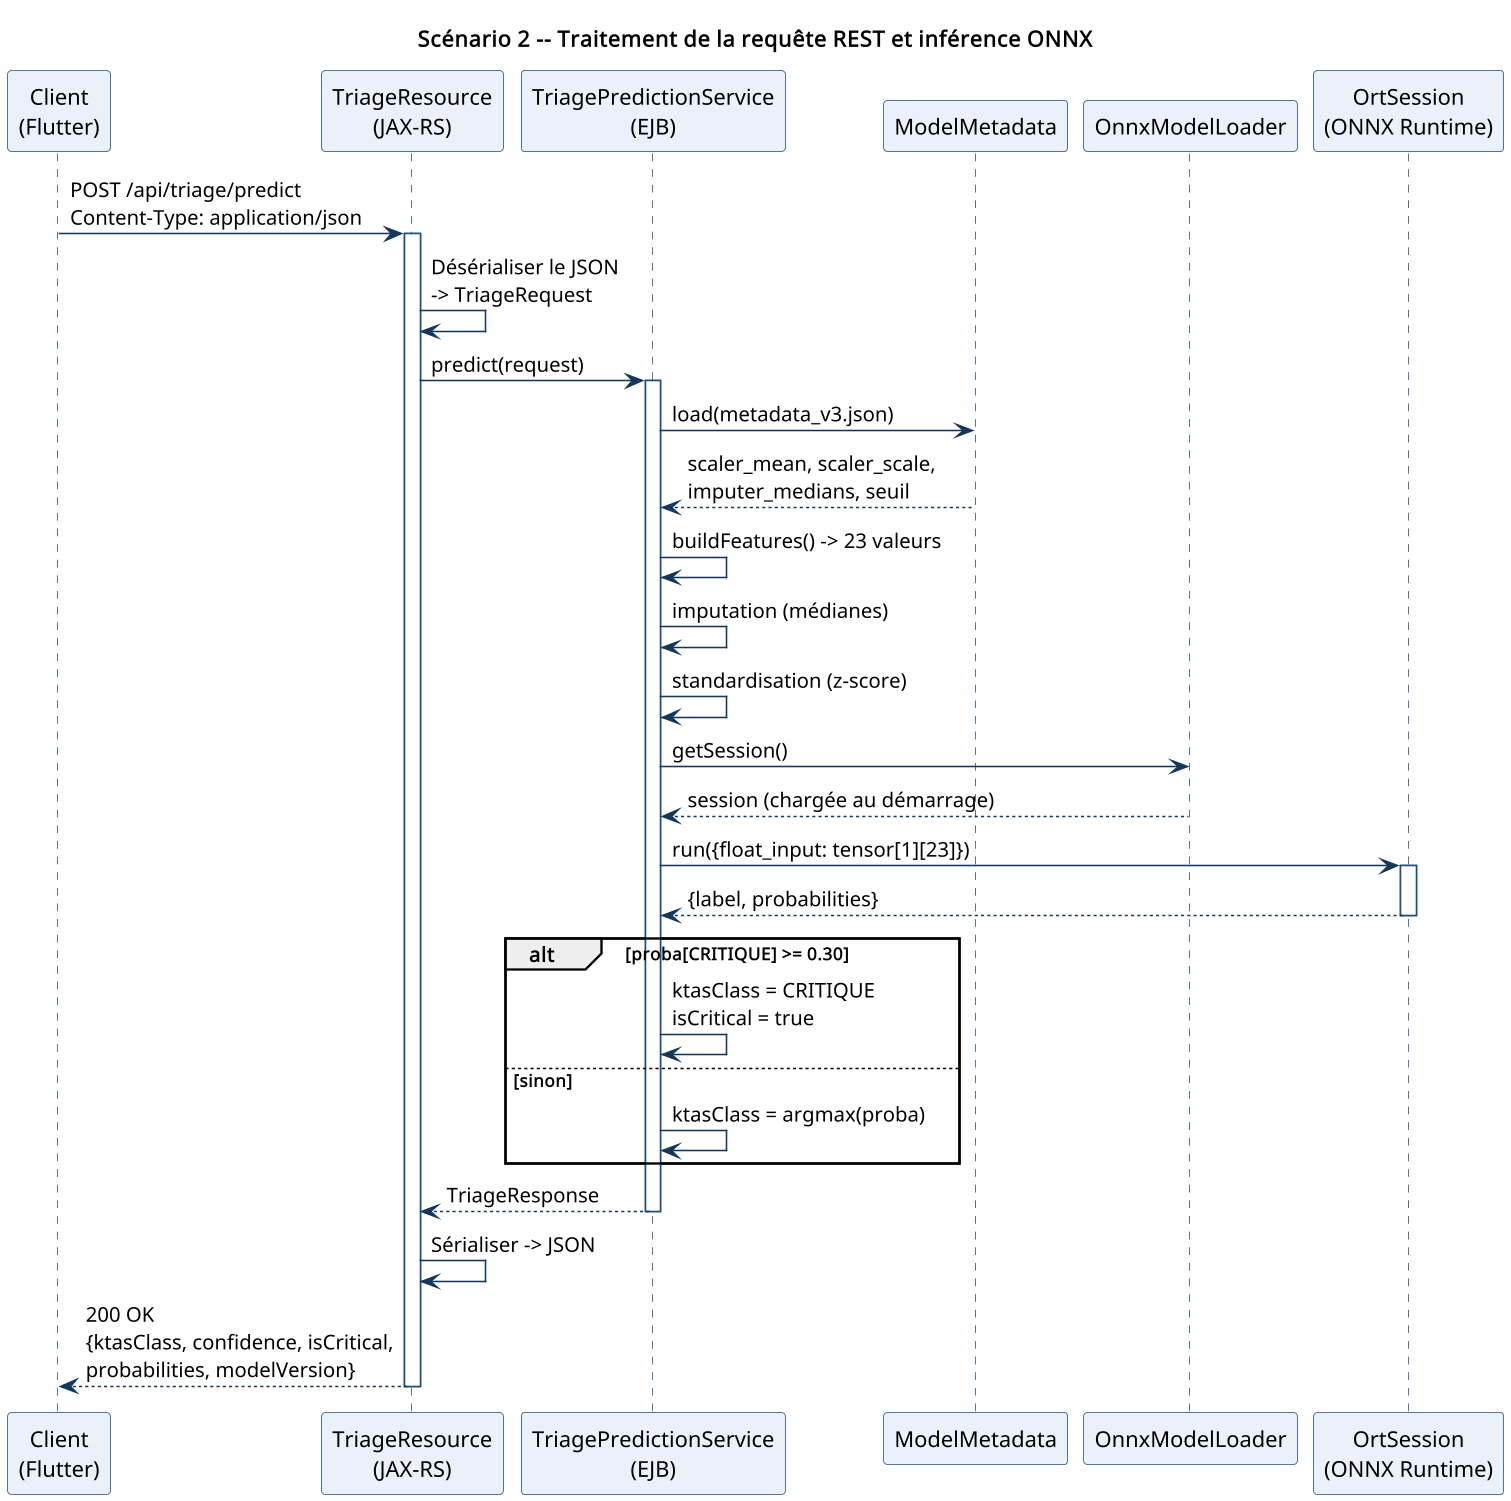
\includegraphics[width=\textwidth]{images/seq_rest.png}
\caption{Scénario 2 -- Traitement de la requête REST et inférence ONNX.}
\label{fig:seqrest}
\end{figure}

\noindent Après désérialisation du JSON en \texttt{TriageRequest}, le service charge les
métadonnées (\texttt{ModelMetadata}), construit les 23 caractéristiques, applique l'imputation par
médianes puis la standardisation z-score. Il récupère ensuite la session auprès du chargeur et
exécute l'inférence sur un tenseur de forme $[1][23]$. Le fragment \texttt{alt} formalise la
règle de décision orientée sécurité : si la probabilité de la classe \textsc{Critique} atteint le
seuil de 0,30, le patient est classé \textsc{Critique} et \texttt{isCritical} est positionné à
vrai ; sinon, la classe retenue est celle de probabilité maximale. La réponse JSON consolide
l'ensemble des informations (classe, confiance, probabilités, version du modèle).

\subsection{Scénario 3 : validation clinique et historisation}
Le troisième scénario (figure~\ref{fig:seqvalid}) illustre l'intervention du médecin, qui valide
ou corrige la proposition, ainsi que l'historisation de la décision finale.

\begin{figure}[h]
\centering
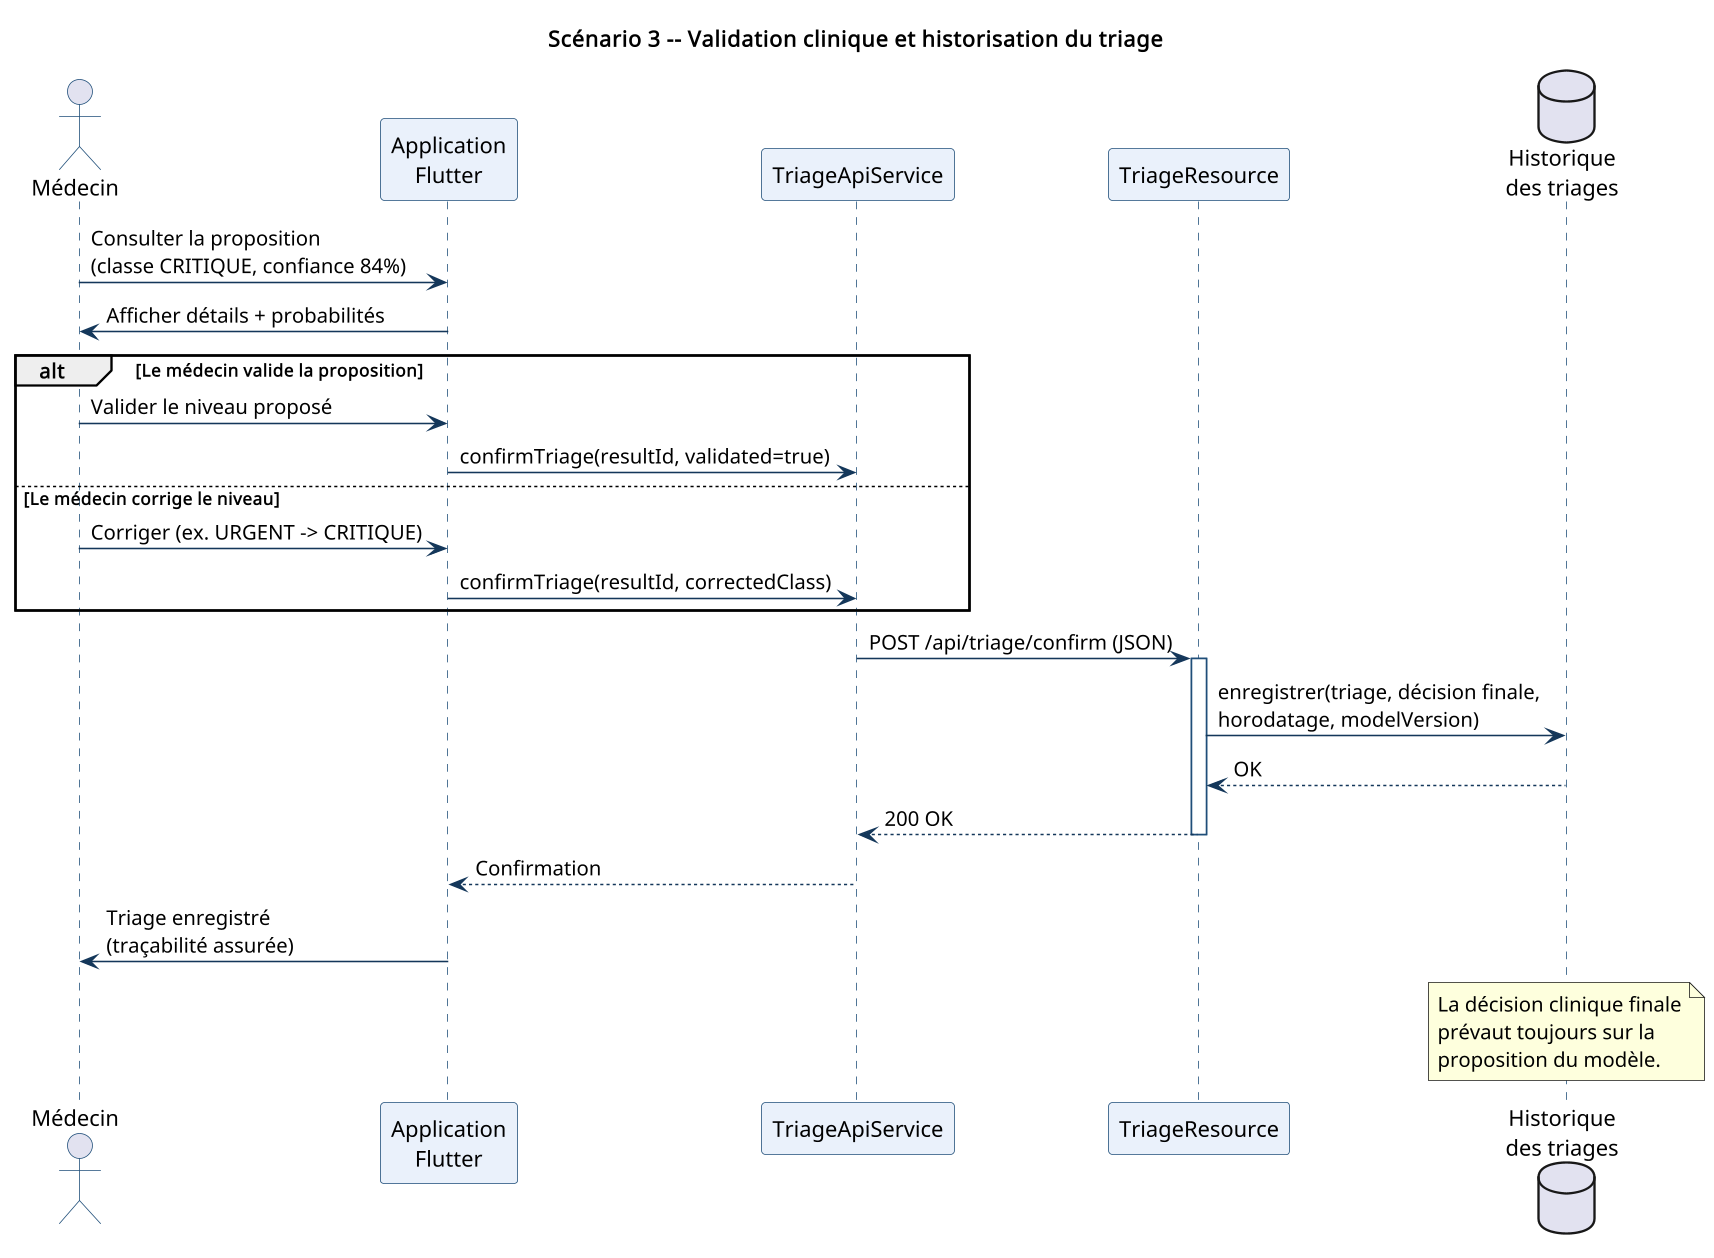
\includegraphics[width=\textwidth]{images/seq_validation.png}
\caption{Scénario 3 -- Validation clinique et historisation du triage.}
\label{fig:seqvalid}
\end{figure}

\noindent Le médecin consulte la proposition assortie des probabilités. Le fragment \texttt{alt}
distingue deux issues : la validation du niveau proposé ou sa correction (par exemple le passage
d'\textsc{Urgent} à \textsc{Critique}). Dans les deux cas, la décision est transmise via
\texttt{POST /api/triage/confirm} et enregistrée dans l'historique des triages avec son
horodatage et la version du modèle. La note finale du diagramme rappelle le principe cardinal de
QuickTriage : \textbf{la décision clinique finale prévaut toujours sur la proposition du modèle}.
Ce scénario matérialise ainsi l'exigence de traçabilité et le positionnement du système comme
simple aide à la décision.

\section*{Conclusion du chapitre}
Ce chapitre a formalisé la conception détaillée de QuickTriage au moyen de la modélisation UML :
le diagramme de cas d'utilisation a clarifié les interactions des acteurs, le diagramme de classes
a exposé la structure statique des couches backend et frontend, et les trois diagrammes de séquence
ont décrit le comportement dynamique du système sur des scénarios représentatifs. Ces modèles
établissent un pont rigoureux entre l'architecture du chapitre précédent et l'implémentation
concrète, objet du chapitre suivant.

\chapter{Implémentation et Démonstration}

\section*{Introduction du chapitre}
Ce dernier chapitre concrétise la conception en présentant la réalisation effective de
QuickTriage. Nous décrivons d'abord l'environnement et la pile technologique de développement,
puis l'implémentation du pipeline d'apprentissage automatique (préparation des données,
optimisation, calibration, résultats). Nous détaillons ensuite l'intégration du modèle dans le
backend J2EE à travers ses composants Java et l'échange REST. Le chapitre se termine par une
démonstration de la solution et une synthèse des artefacts produits.

\section{Environnement et pile technologique}

\subsection{Outils et versions}
La réalisation de QuickTriage a mobilisé un ensemble cohérent de technologies, réparties sur les
trois couches. Le tableau~\ref{tab:stack} en récapitule la pile, avec les versions retenues.

\begin{table}[h]
\centering
\renewcommand{\arraystretch}{1.35}
\begin{tabular}{p{3cm} p{5cm} p{5.5cm}}
\toprule
\textbf{Couche} & \textbf{Technologie} & \textbf{Rôle} \\
\midrule
\multirow{6}{*}{Apprentissage}
 & Python 3 & Langage du pipeline ML \\
 & pandas, NumPy & Manipulation des données \\
 & scikit-learn & Prétraitement, métriques, SMOTE (\textit{imbalanced-learn}) \\
 & XGBoost & Modèle de classification \\
 & Optuna & Optimisation des hyperparamètres \\
 & ONNX / skl2onnx & Export du modèle interopérable \\
\midrule
\multirow{4}{*}{Backend}
 & Jakarta EE & Plateforme d'entreprise \\
 & WildFly 10 & Serveur d'application \\
 & JAX-RS / EJB & API REST et logique métier \\
 & ONNX Runtime 1.18.0 & Moteur d'inférence (\texttt{com.microsoft.onnxruntime}) \\
\midrule
\multirow{2}{*}{Frontend}
 & Android (Android Studio) & Application mobile (Java/Kotlin) \\
 & Retrofit / OkHttp & Consommation de l'API REST \\
\midrule
Outillage & Maven, Git & Construction et gestion de versions \\
\bottomrule
\end{tabular}
\caption{Pile technologique de QuickTriage.}
\label{tab:stack}
\end{table}

\section{Implémentation du pipeline d'apprentissage automatique}

\subsection{Préparation et augmentation des données}
Le jeu de données \textit{KTAS Emergency Triage} comporte initialement 1~267 patients réels,
fortement déséquilibrés entre les classes. Pour corriger ce déséquilibre, une stratégie
d'augmentation hybride a été mise en œuvre, combinant la génération de patients synthétiques
calibrés sur les distributions réelles et l'algorithme SMOTE. Le résultat est un jeu équilibré de
3~000 patients, soit 600 par classe métier. Le listing~\ref{lst:smote} illustre le principe du
rééquilibrage par SMOTE avec un nombre de voisins adaptatif.

\begin{listing}[H]
\begin{minted}[bgcolor=bg,fontsize=\small,linenos]{python}
from imblearn.over_sampling import SMOTE
from collections import Counter

# Determination d'un k_neighbors adaptatif (robuste aux petites classes)
counts = Counter(y_train)
min_class_size = min(counts.values())
k_neighbors = max(1, min(5, min_class_size - 1))

smote = SMOTE(random_state=42, k_neighbors=k_neighbors)
X_balanced, y_balanced = smote.fit_resample(X_train, y_train)

print("Distribution apres reequilibrage :", Counter(y_balanced))
# -> {CRITIQUE: 600, URGENT: 600, NON_URGENT: 600}
\end{minted}
\caption{Rééquilibrage des classes par SMOTE avec \texttt{k\_neighbors} adaptatif.}
\label{lst:smote}
\end{listing}

\subsection{Optimisation des hyperparamètres avec Optuna}
Le modèle XGBoost a été optimisé par Optuna sur \textbf{80 essais}. La fonction objectif maximise
le F1-score pondéré obtenu en validation croisée. Le listing~\ref{lst:optuna} en présente une forme
simplifiée.

\begin{listing}[H]
\begin{minted}[bgcolor=bg,fontsize=\small,linenos]{python}
import optuna
from xgboost import XGBClassifier
from sklearn.model_selection import cross_val_score

def objective(trial):
    params = {
        "n_estimators":  trial.suggest_int("n_estimators", 100, 600),
        "max_depth":     trial.suggest_int("max_depth", 3, 10),
        "learning_rate": trial.suggest_float("learning_rate", 1e-3, 0.3, log=True),
        "subsample":     trial.suggest_float("subsample", 0.6, 1.0),
        "colsample_bytree": trial.suggest_float("colsample_bytree", 0.6, 1.0),
    }
    model = XGBClassifier(**params, eval_metric="mlogloss", random_state=42)
    score = cross_val_score(model, X_balanced, y_balanced,
                            cv=5, scoring="f1_weighted").mean()
    return score

study = optuna.create_study(direction="maximize")
study.optimize(objective, n_trials=80)
print("Meilleur essai :", study.best_trial.number)   # -> 64
print("Meilleurs parametres :", study.best_params)
\end{minted}
\caption{Optimisation des hyperparamètres de XGBoost avec Optuna (80 essais).}
\label{lst:optuna}
\end{listing}

\noindent Le meilleur essai (\textbf{n\textsuperscript{o}~64}) retient les hyperparamètres
suivants : \texttt{n\_estimators}~=~458, \texttt{max\_depth}~=~7 et
\texttt{learning\_rate}~$\approx$~0,0113. Ces valeurs traduisent un modèle relativement profond et
nombreux en arbres, mais à pas d'apprentissage faible, gage de stabilité.

\subsection{Calibration du seuil orientée sécurité patient}
Conformément au parti pris de minimiser le sous-triage, le seuil de décision de la classe
\textsc{Critique} a été abaissé à \textbf{0,30} au lieu de la règle usuelle de l'\textit{argmax}.
Concrètement, dès que la probabilité estimée d'appartenance à la classe \textsc{Critique} atteint
0,30, le patient est classé comme critique. Ce réglage privilégie délibérément le rappel des cas
graves au prix d'un léger sur-triage, jugé acceptable d'un point de vue clinique.

\subsection{Résultats et évaluation}
Le tableau~\ref{tab:metrics} synthétise les performances du modèle final. L'évaluation met
l'accent sur la classe \textsc{Critique}, dont le rappel constitue l'indicateur de sécurité
déterminant.

\begin{table}[h]
\centering
\renewcommand{\arraystretch}{1.35}
\begin{tabular}{p{6cm} c}
\toprule
\textbf{Métrique} & \textbf{Valeur} \\
\midrule
Exactitude globale (\textit{accuracy}) & 73,8~\% \\
F1-score pondéré (\textit{weighted}) & 0,729 \\
Rappel classe \textsc{Critique} & 83,9~\% \\
F1-score classe \textsc{Critique} & 0,80 \\
Seuil de décision \textsc{Critique} & 0,30 \\
\bottomrule
\end{tabular}
\caption{Performances du modèle XGBoost final de QuickTriage.}
\label{tab:metrics}
\end{table}

\begin{successbox}
Avec un \textbf{rappel de 83,9~\%} sur la classe \textsc{Critique}, le modèle identifie
correctement la grande majorité des patients en danger vital, ce qui constitue l'objectif
prioritaire d'un système d'aide au triage.
\end{successbox}

\noindent La matrice de confusion (figure~\ref{fig:confusion}) détaille la répartition des
prédictions par classe et confirme la rareté des erreurs de sous-triage les plus graves
(patients critiques classés non urgents).

\figplaceholder{[Figure 6.1 -- Matrice de confusion du modèle final sur le jeu de test
(classes CRITIQUE, URGENT, NON\_URGENT). À insérer : image exportée depuis le notebook
d'évaluation.]}
\begin{figure}[h]
\centering
\caption{Matrice de confusion du modèle final.}
\label{fig:confusion}
\end{figure}

\subsection{Export ONNX}
Une fois le modèle entraîné et validé, il est exporté au format ONNX afin d'être consommé par le
backend Java. Le listing~\ref{lst:onnx} montre l'export via \texttt{skl2onnx}. L'artefact produit,
\texttt{triage\_final\_v3.onnx}, occupe environ 139~Ko.

\begin{listing}[H]
\begin{minted}[bgcolor=bg,fontsize=\small,linenos]{python}
from skl2onnx import convert_sklearn
from skl2onnx.common.data_types import FloatTensorType

initial_type = [("float_input", FloatTensorType([None, 23]))]
onnx_model = convert_sklearn(best_model, initial_types=initial_type,
                             options={type(best_model): {"zipmap": False}})

with open("triage_final_v3.onnx", "wb") as f:
    f.write(onnx_model.SerializeToString())
\end{minted}
\caption{Export du modèle au format ONNX (entrée \texttt{float\_input} de dimension 23).}
\label{lst:onnx}
\end{listing}

\section{Intégration du modèle dans le backend J2EE}

\subsection{Chargement du modèle : \texttt{OnnxModelLoader}}
Le bean \texttt{OnnxModelLoader} charge le modèle une seule fois au démarrage du serveur grâce aux
annotations \texttt{@Singleton} et \texttt{@Startup}. La session ONNX est ensuite réutilisée pour
toutes les inférences (listing~\ref{lst:loader}).

\begin{listing}[H]
\begin{minted}[bgcolor=bg,fontsize=\small,linenos,breaklines]{java}
@Singleton
@Startup
public class OnnxModelLoader {

    private OrtEnvironment env;
    private OrtSession session;

    @PostConstruct
    public void init() {
        try {
            env = OrtEnvironment.getEnvironment();
            byte[] model = getClass().getResourceAsStream("/triage_final_v3.onnx")
                                     .readAllBytes();
            session = env.createSession(model, new OrtSession.SessionOptions());
        } catch (Exception e) {
            throw new IllegalStateException("Echec du chargement du modele ONNX", e);
        }
    }

    public OrtSession getSession() {
        return session;
    }

    @PreDestroy
    public void close() throws Exception {
        if (session != null) session.close();
        if (env != null) env.close();
    }
}
\end{minted}
\caption{Chargement unique du modèle ONNX au démarrage (\texttt{OnnxModelLoader}).}
\label{lst:loader}
\end{listing}

\subsection{Logique métier : \texttt{TriagePredictionService}}
L'EJB \texttt{@Stateless} \texttt{TriagePredictionService} construit le vecteur de
caractéristiques, applique le prétraitement issu des métadonnées, exécute l'inférence et applique
le seuil de criticité (listing~\ref{lst:service}).

\begin{listing}[H]
\begin{minted}[bgcolor=bg,fontsize=\small,linenos,breaklines]{java}
@Stateless
public class TriagePredictionService {

    @Inject
    private OnnxModelLoader modelLoader;

    private final ModelMetadata meta = ModelMetadata.load("/metadata_v3.json");

    public TriageResponse predict(TriageRequest req) throws Exception {
        float[] features = normalize(buildFeatures(req));

        OrtSession session = modelLoader.getSession();
        OrtEnvironment env = OrtEnvironment.getEnvironment();
        OnnxTensor input = OnnxTensor.createTensor(env, new float[][]{features});

        try (OrtSession.Result result =
                 session.run(Collections.singletonMap("float_input", input))) {
            float[] proba = extractProbabilities(result);
            return applyThreshold(proba);
        }
    }

    private TriageResponse applyThreshold(float[] proba) {
        TriageResponse resp = new TriageResponse();
        if (proba[KtasClass.CRITIQUE.ordinal()] >= meta.getSeuilCritique()) {
            resp.setKtasClass(KtasClass.CRITIQUE);
            resp.setCritical(true);
        } else {
            resp.setKtasClass(KtasClass.values()[argmax(proba)]);
        }
        resp.setProbabilities(toMap(proba));
        resp.setModelVersion(meta.getModelVersion());
        return resp;
    }
}
\end{minted}
\caption{Logique métier de prédiction et application du seuil (\texttt{TriagePredictionService}).}
\label{lst:service}
\end{listing}

\subsection{Exposition REST : \texttt{TriageResource}}
La ressource JAX-RS \texttt{TriageResource} expose le point d'entrée \texttt{POST
/api/triage/predict} et délègue le traitement au service (listing~\ref{lst:resource}).

\begin{listing}[H]
\begin{minted}[bgcolor=bg,fontsize=\small,linenos,breaklines]{java}
@Path("/api/triage")
@Produces(MediaType.APPLICATION_JSON)
@Consumes(MediaType.APPLICATION_JSON)
public class TriageResource {

    @Inject
    private TriagePredictionService predictionService;

    @POST
    @Path("/predict")
    public Response predict(TriageRequest request) {
        try {
            TriageResponse response = predictionService.predict(request);
            return Response.ok(response).build();
        } catch (Exception e) {
            return Response.status(Response.Status.INTERNAL_SERVER_ERROR)
                           .entity("Erreur lors de la prediction").build();
        }
    }
}
\end{minted}
\caption{Point d'entrée REST de prédiction (\texttt{TriageResource}).}
\label{lst:resource}
\end{listing}

\subsection{Dépendance Maven}
L'intégration du moteur d'inférence repose sur la dépendance Maven présentée au
listing~\ref{lst:maven}.

\begin{listing}[H]
\begin{minted}[bgcolor=bg,fontsize=\small]{xml}
<dependency>
    <groupId>com.microsoft.onnxruntime</groupId>
    <artifactId>onnxruntime</artifactId>
    <version>1.18.0</version>
</dependency>
\end{minted}
\caption{Dépendance Maven pour ONNX Runtime.}
\label{lst:maven}
\end{listing}

\subsection{Format d'échange REST}
L'échange entre le client Android et le backend repose sur JSON. Le listing~\ref{lst:json}
présente un exemple de requête et la réponse correspondante pour un patient critique.

\begin{listing}[H]
\begin{minted}[bgcolor=bg,fontsize=\small]{json}
// Requete : POST /api/triage/predict
{
  "age": 72, "mental": 3, "nrsPain": 8,
  "sbp": 85, "dbp": 50, "hr": 124, "rr": 28,
  "bt": 38.9, "saturation": 90, "arrivalMode": 3
}

// Reponse : 200 OK
{
  "ktasClass": "CRITIQUE",
  "ktasLevels": "1-2",
  "delaiMax": 15,
  "confidence": 0.84,
  "isCritical": true,
  "probabilities": { "CRITIQUE": 0.84, "URGENT": 0.12, "NON_URGENT": 0.04 },
  "modelVersion": "v3"
}
\end{minted}
\caption{Exemple d'échange REST JSON (requête et réponse).}
\label{lst:json}
\end{listing}

\section{Synthèse des artefacts produits}
Le tableau~\ref{tab:artefacts} récapitule les principaux artefacts de la chaîne QuickTriage.

\begin{table}[h]
\centering
\renewcommand{\arraystretch}{1.35}
\begin{tabular}{p{4.5cm} p{3cm} p{6cm}}
\toprule
\textbf{Artefact} & \textbf{Type} & \textbf{Description} \\
\midrule
\texttt{triage\_final\_v3.onnx} & Modèle (139 Ko) & Modèle XGBoost exporté, consommé par le backend \\
\texttt{metadata\_v3.json} & Métadonnées & Scaler, médianes d'imputation, seuil, version \\
\texttt{OnnxModelLoader.java} & Backend & Chargement unique du modèle (Singleton) \\
\texttt{TriagePredictionService.java} & Backend & Logique métier d'inférence (EJB) \\
\texttt{TriageResource.java} & Backend & Point d'entrée REST (JAX-RS) \\
Application Android & Frontend & Saisie et restitution mobile \\
\bottomrule
\end{tabular}
\caption{Principaux artefacts de la solution QuickTriage.}
\label{tab:artefacts}
\end{table}

\section{Démonstration}
Cette section illustre le fonctionnement de l'application mobile sur un parcours type. Les captures
d'écran (à insérer) présentent successivement l'écran de saisie des constantes, l'écran de
résultat pour un cas critique et l'écran de résultat pour un cas non urgent.

\figplaceholder{[Figure 6.2 -- Écran de saisie des constantes vitales dans l'application Android.]}
\begin{figure}[h]
\centering
\caption{Application QuickTriage -- écran de saisie des constantes.}
\label{fig:demo-saisie}
\end{figure}

\figplaceholder{[Figure 6.3 -- Écran de résultat pour un patient CRITIQUE (bandeau rouge,
alerte de criticité, délai immédiat, confiance et probabilités).]}
\begin{figure}[h]
\centering
\caption{Application QuickTriage -- résultat pour un cas critique.}
\label{fig:demo-critique}
\end{figure}

\figplaceholder{[Figure 6.4 -- Écran de résultat pour un patient NON\_URGENT (bandeau vert).]}
\begin{figure}[h]
\centering
\caption{Application QuickTriage -- résultat pour un cas non urgent.}
\label{fig:demo-nonurgent}
\end{figure}

\noindent La démonstration confirme le comportement attendu de bout en bout : la saisie des
constantes déclenche un appel à l'API, l'inférence est restituée en une fraction de seconde et le
code couleur permet une lecture immédiate de la priorité. Le cas critique déclenche bien l'alerte
\texttt{isCritical}, conformément à la règle de seuil calibrée.

\section*{Conclusion du chapitre}
Ce chapitre a présenté la réalisation concrète de QuickTriage : la pile technologique,
l'implémentation du pipeline d'apprentissage (augmentation hybride, optimisation Optuna,
calibration orientée sécurité, export ONNX), l'intégration du modèle dans le backend J2EE via ses
trois composants Java, l'échange REST JSON, ainsi qu'une démonstration de l'application mobile. La
solution couvre ainsi l'intégralité de la chaîne, de la donnée brute jusqu'à l'aide à la décision
restituée au soignant. La conclusion générale dresse le bilan de ce travail et en esquisse les
perspectives.


%------------ Liste of listings----------------
%\renewcommand\listoflistingscaption{Liste des codes source}
%\listoflistings
\newpage
\chapter*{Conclusion Générale et Perspectives}
\addcontentsline{toc}{chapter}{Conclusion Générale et Perspectives}
Ce projet de fin d'année a permis de concevoir et de réaliser \textbf{QuickTriage}, un système
intelligent d'aide au triage des patients aux urgences, couvrant l'intégralité de la chaîne, depuis
la donnée brute jusqu'à l'application mobile destinée au personnel soignant.

\medskip
\noindent\textbf{Bilan du travail réalisé.} Le projet a d'abord posé le cadre clinique et la
problématique du triage, puis dressé un état de l'art des échelles normalisées (CTAS, ESI, MTS,
KTAS) et des approches d'apprentissage automatique appliquées au triage. Sur cette base, les besoins
fonctionnels et non-fonctionnels ont été formalisés, puis traduits en une architecture en trois
couches faiblement couplées : un pipeline d'apprentissage en Python, un backend Jakarta EE exposant
le modèle au format ONNX via une API REST JAX-RS, et un frontend mobile Flutter. La modélisation UML
(cas d'utilisation, classes, séquences) a précisé la conception, avant que l'implémentation ne la
concrétise.

\medskip
\noindent\textbf{Principaux résultats.} Le modèle XGBoost final, optimisé par Optuna et entraîné sur
un jeu de données rééquilibré par augmentation hybride, atteint une exactitude de 73,8~\%, un
F1-score pondéré de 0,729 et, surtout, un rappel de 83,9~\% sur la classe \textsc{Critique}. Ce
dernier résultat, obtenu grâce à une calibration du seuil de décision à 0,30, traduit le parti pris
fondamental du projet : \textbf{minimiser le sous-triage} pour préserver la sécurité des patients en
danger vital. La détection et la correction d'une fuite de données ont par ailleurs garanti
l'honnêteté et la généralisabilité des performances annoncées.

\medskip
\noindent\textbf{Limites.} Plusieurs limites doivent être soulignées. Les performances restent
contraintes par la taille et la nature du jeu de données initial (1~267 patients réels) ; le recours
à l'augmentation synthétique, bien que nécessaire, introduit une part d'artificialité dans les
données d'entraînement. De plus, le système n'a pas été validé en conditions cliniques réelles, et
l'historisation comme la sécurisation complète (authentification, HTTPS de bout en bout) relèvent
encore d'une mise en production à venir.

\medskip
\noindent\textbf{Perspectives.} Plusieurs axes d'amélioration se dégagent :
\begin{itemize}
  \item \textbf{Enrichissement des données} : intégrer des jeux de données réels plus volumineux et
  multicentriques, afin de réduire la dépendance à l'augmentation synthétique et d'améliorer la
  généralisation.
  \item \textbf{Validation clinique} : conduire une évaluation prospective auprès de soignants, pour
  mesurer l'apport réel de l'outil et son acceptabilité sur le terrain.
  \item \textbf{Explicabilité} : intégrer des méthodes d'explication (par exemple SHAP) afin de
  rendre transparentes les raisons d'une prédiction et de renforcer la confiance des soignants.
  \item \textbf{Sécurité et conformité} : finaliser l'authentification, le chiffrement de bout en
  bout et la conformité réglementaire (RGPD) pour un déploiement en production.
  \item \textbf{Apprentissage continu} : exploiter les décisions validées et corrigées par les
  médecins (historisées) pour réentraîner périodiquement le modèle et l'améliorer dans le temps.
\end{itemize}

\medskip
\noindent En définitive, QuickTriage démontre la faisabilité d'une chaîne complète, interopérable et
orientée sécurité patient pour l'aide au triage. Au-delà de ses résultats techniques, le projet
illustre une démarche d'ingénierie rigoureuse, attentive aux pièges méthodologiques de la science des
données et à l'impératif éthique de placer le jugement clinique du soignant au cœur de la décision.


\newpage
\bibliographystyle{plain}
\bibliography{refs}

\newpage
\chapter*{Annexes}
\addcontentsline{toc}{chapter}{Annexes}
\section*{Annexe A -- Variables d'entrée du modèle}
\addcontentsline{toc}{section}{Annexe A -- Variables d'entrée du modèle}

Le tableau~\ref{tab:annexe-features} présente les principales constantes vitales et variables
utilisées en entrée du modèle de triage.

\begin{table}[h]
\centering
\renewcommand{\arraystretch}{1.3}
\begin{tabular}{p{3.2cm} p{3cm} p{7cm}}
\toprule
\textbf{Variable} & \textbf{Unité / Type} & \textbf{Description} \\
\midrule
\texttt{age}        & années & Âge du patient \\
\texttt{mental}     & catégoriel & État mental (alerte, voix, douleur, inconscient) \\
\texttt{nrsPain}    & 0--10 & Intensité de la douleur (échelle numérique NRS) \\
\texttt{sbp}        & mmHg & Pression artérielle systolique \\
\texttt{dbp}        & mmHg & Pression artérielle diastolique \\
\texttt{hr}         & bpm & Fréquence cardiaque \\
\texttt{rr}         & /min & Fréquence respiratoire \\
\texttt{bt}         & \textdegree C & Température corporelle \\
\texttt{saturation} & \% & Saturation pulsée en oxygène (SpO\textsubscript{2}) \\
\texttt{arrivalMode}& catégoriel & Mode d'arrivée aux urgences \\
\bottomrule
\end{tabular}
\caption{Principales variables d'entrée du modèle QuickTriage.}
\label{tab:annexe-features}
\end{table}

\section*{Annexe B -- Structure des métadonnées de prétraitement}
\addcontentsline{toc}{section}{Annexe B -- Structure des métadonnées de prétraitement}

Le fichier \texttt{metadata\_v3.json} externalise les paramètres de prétraitement chargés par le
backend au démarrage. Sa structure est la suivante :

\begin{listing}[H]
\begin{minted}[bgcolor=bg,fontsize=\small]{json}
{
  "model_version": "v3",
  "feature_order": ["age", "mental", "nrsPain", "sbp", "dbp",
                    "hr", "rr", "bt", "saturation", "arrivalMode", "..."],
  "imputer_medians": [/* mediane par feature */],
  "scaler_mean":     [/* moyenne par feature (StandardScaler) */],
  "scaler_scale":    [/* ecart-type par feature (StandardScaler) */],
  "seuil_critique":  0.30,
  "classes": ["CRITIQUE", "URGENT", "NON_URGENT"]
}
\end{minted}
\caption{Structure du fichier \texttt{metadata\_v3.json}.}
\label{lst:annexe-meta}
\end{listing}

\section*{Annexe C -- Correspondance KTAS / classes métier}
\addcontentsline{toc}{section}{Annexe C -- Correspondance KTAS / classes métier}

\begin{table}[h]
\centering
\renewcommand{\arraystretch}{1.4}
\begin{tabular}{p{3.2cm} p{2.5cm} p{6.5cm}}
\toprule
\textbf{Classe métier} & \textbf{Niveaux KTAS} & \textbf{Délai de prise en charge} \\
\midrule
\textcolor{qtcritique}{\textbf{CRITIQUE}}     & KTAS 1--2 & Immédiate ($<$ 15 min) \\
\textcolor{qturgent}{\textbf{URGENT}}         & KTAS 3    & Rapide \\
\textcolor{qtnonurgent}{\textbf{NON\_URGENT}} & KTAS 4--5 & Différée \\
\bottomrule
\end{tabular}
\caption{Correspondance entre les niveaux KTAS et les classes métier de QuickTriage.}
\label{tab:annexe-ktas}
\end{table}

\section*{Annexe D -- Hyperparamètres optimaux du modèle}
\addcontentsline{toc}{section}{Annexe D -- Hyperparamètres optimaux du modèle}

Le tableau~\ref{tab:annexe-hp} récapitule les hyperparamètres du meilleur essai Optuna
(essai n\textsuperscript{o}~64) retenus pour le modèle XGBoost final.

\begin{table}[h]
\centering
\renewcommand{\arraystretch}{1.3}
\begin{tabular}{p{5cm} c}
\toprule
\textbf{Hyperparamètre} & \textbf{Valeur} \\
\midrule
\texttt{n\_estimators}  & 458 \\
\texttt{max\_depth}     & 7 \\
\texttt{learning\_rate} & $\approx$ 0,0113 \\
Nombre d'essais Optuna  & 80 \\
Meilleur essai          & n\textsuperscript{o} 64 \\
\bottomrule
\end{tabular}
\caption{Hyperparamètres optimaux du modèle XGBoost final.}
\label{tab:annexe-hp}
\end{table}


\end{document}
